\RequirePackage[l2tabu,orthodox]{nag}
\documentclass[11pt]{book}
\usepackage{calc}
\usepackage{xcolor}
\usepackage[utf8]{inputenc}
\usepackage{amsmath}
\usepackage{amssymb}
\usepackage{braket}
\usepackage{graphicx}
\usepackage{subfig}
\usepackage{array}
\usepackage{caption}
\usepackage[nottoc]{tocbibind}

\usepackage{comment}
\usepackage{todonotes}
\usepackage[hyperfootnotes=false,hidelinks=true]{hyperref}
\usepackage{natbib}
\newcommand{\markup}[2][red]{\textcolor{#1}{#2}}
\usepackage{algorithm2e}
\usepackage{pdfpages}

%%%%%%%%%%%%%%%%%%%%%%%%%%%%%%%%%%%%%%%%%%%%%%%%%%%%%%%%%%%%%%%%%%%%%%%%%%%%%%%%%%%%%
\begin{document}

\frontmatter

\begin{titlepage}

\setlength\oddsidemargin{(\paperwidth-\textwidth)/2 - 1in}
\setlength\topmargin{(\paperheight-\textheight
-\headheight-\headsep-\footskip)/2 - 1in}

\begin{center}
\vspace*{-2. cm}

\includegraphics[width=4.5cm]{Figs/Logo_Universita_Padova.png}
\vspace*{1 cm}

{\bfseries{\huge Universit\`a degli studi di Padova} }
\hrule

\vspace{1 cm}

{\Large Dipartimento di Fisica e Astronomia  `` Galileo Galilei "} 

\vspace{0.5cm}

{\Large Dipartimento di Ingegneria dell'Informazione} 
\vspace{1cm}

{\Large Corso di Laurea Magistrale in} 
{\Large Fisica}

\vspace{1.5 cm}

{\LARGE{\bfseries {Large--scale Classical Simulation of Quantum Systems Using the Trotter--Suzuki Decomposition}}} 
\end{center}

\vfill
\raggedright     
%\large{Controrelatore: Francesco Ancilotto}  \\
%\vspace{0.08cm} 
\large{Relatore esterno: Antonio Acín}  \\
\vspace{0.08cm}
\large{Correlatore esterno: Peter Wittek}  \\
\vspace{0.08 cm}
\large{Relatore interno: Giuseppe Vallone}  \\
\vspace{0.08cm}

\raggedleft
\large{Laureando}

\large{Luca Calderaro} 

\vspace{2cm}
\begin{center}
{\large{ Anno Accademico 2014/2015}}
\end{center}
\vspace{-1.5cm}

\end{titlepage}

\thispagestyle{empty}
\begin{center}
\newpage

\vspace*{5cm}

\Large\textit{Dedicated to Sara.} 
\end{center}


\chapter*{Abstract}
Many theoretical studies and experimental results rely on the use of numerical analysis for the solution of the Schr\"odinger equation. Indeed, for nontrivial quantum systems, a complete solution of the dynamics is difficult to achieve analytically. We extended the implementation of a highly optimized solver to simulate the evolution of a wave function on a 2D lattice. We also implemented the imaginary time evolution to approximate the ground state. The dynamics of the system is now described by an Hamiltonian that includes an external potential and a contact interaction term. The algorithm is based on the second order Trotter--Suzuki approximation and it is implemented on CPU and GPU kernels that run efficiently on a cluster. We proved the accuracy of the code solving the Gross-Pitaevskii equation for a Bose-Einstein condensate and reproducing the experimental results, obtained at NIST, about the soliton dynamics in a cloud of sodium atoms. The code is available under an open source license, and it is exposed as an application program interface. The code is also accessible in Python and MATLAB. Future development of the code include the extension to a 3D lattice, whereas the actual implementation can already find applications in ultracold atom physics.

\thispagestyle{empty}
\chapter*{Acknowledgement}

\begin{figure}[h!]
\centering
   
\includegraphics[width=5cm]{Figs/logo_icfo.png}
\end{figure}

\noindent This Thesis project has been carried out during my Erasmus internship at ICFO--The Institute of Photonic Sciences in Barcelona. Special thanks are given to my supervisors Peter Wittek and Toni Acín for having me in their research group and for all the great support they gave me.
Also, I like to thank Pietro Massignan for his invaluable support in the physical application of the code.
Thanks to all the ICFOnians who made my internship an enjoyable and productive experience. 

\vspace{1cm}

\noindent Thanks to my parents and my sister for having raised me and always sustained me in my aspirations.

\thispagestyle{empty}
%\pagenumbering{Roman}
\tableofcontents

\listoffigures

\mainmatter

\chapter{Introduction}
Since the creation of the first electronic digital computing device\footnote{John Vincent Atanasoff and Clifford Berry created the first electronic non-programmable, digital computing device, the Atanasoff–Berry Computer, from 1937 to 1942}, physicists have used computers as a valuable tools for their research. The study and the implementation of numerical methods to solve physical problem led to the growth of a new field of physics called computational physics. It is not surprising that this field of physics has branches in every major field in physics: from computational mechanics to computational astrophysics, from computational condensed matter to computational particle physics.
%put some references?
 Mathematical models, developed to accurately describe natural phenomena, are very often difficult to solve analytically. The prescription to build up a physics model requires to define the energy of the system, which contains the interactions between the components of the system and the kinetic of the particles -- when these are allowed to move --. This in turn leads to the action of the system and the equations of motion by means of the least action principle~\citep{LL85}. At this stage, depending on what system is under study, many features can be already found without considering the equations of motion. For instance, the phase transitions of a spin system in the canonical ensemble may be studied considering the partition function which in turn let us calculate observables, like the magnetization as a function of the temperature and the external magnetic field~\citep{Huang28}. These features regards the equilibrium properties of the system and may constitute a rather challenging analytical problem. Even more challenging may be the study of the dynamical properties, in which one has to deal with the equations of motion. In particular, one would have to solve the Cauchy problem, in which the initial state of the system is given along with the equations.

The correctness of a physics model is evaluated comparing its results with the outcomes of the experiment. As we said, it is not always possible to get the results we need from the model by mean of analytical method. A possible approach to tackle these problems is to use algorithm to numerically solve the equations.

Complicated systems lead to numerically intense simulations that require a great amount of computational resources. For this reason, the development of efficient code, able to take advantage of the computational resources available nowadays, is of fundamental importance. A lack in efficiency may lead to long time of execution, that can extend to months or even years, making the simulations impracticable. 

The most powerful computational facilities at our disposal are supercomputers. These machines consist of many single processing units connected with each other to share data. An algorithm can get the most from these machines when it is able to use many processing units at the same time, parallelizing the tasks to be performed. Processing units can be distinguished into two main categories: central processing units (CPUs) and graphic processing units (GPUs). The former dedicate most of their transistor count to improve sequential code performance, while the latter take a different approach housing hundreds of simple execution units which run parallel code. Due to their features, GPUs are gaining popularity in the computational physics field. They are designed to perform simple calculations on large amount of data in parallel. These features can lead to a great speed-up of the execution time with respect to a sequential code implemented on a CPU.

In this work we developed a solver for schr\"odinger equation that scales to	massively parallel computing clusters. We started from the recent work of Wittek and Cucchietti~\citep{Wittek20131165}, in which they extended the single-node parallel kernels in Ref.~\citep{bederian2011boosting} to use distributed resources. We further extended the code implementing the external potential in the Hamiltonian. This allows to simulate a wider range of problems in quantum physics. The implementation is also able to solve the nonlinear Schr\"odinger equation. The code implements cache optimized kernels for both CPUs and GPUs, making it versatile to use on different types of computing resources. These kernels are based on the second order Trotter-Suzuki decomposition~\citep{Suzuki1992387}. The approximation allows the evolution operator to be decomposed in a sequence of operators easy to evaluate.

As application of the code we were able to simulate the evolution of an interacting Bose-Einstein condensate, described by the Gross-Pitaevskii equation. The simulation reproduced the experimental results in Ref.~\citep{DSF00}.

The content of the Thesis is organized in the following way. The second chapter introduces to the Trotter-Suzuki approximation. In the third we explicitly calculate the evolution operator that is implemented in our code. The fourth chapter gives the details of the algorithms used in our code, describing the optimization techniques. The fifth chapter presents the application to the interacting BEC and we compare our results with the experimental study of Ref.~\citep{DSF00}. We conclude summarizing our achievements and outlining the future directions of research.

\chapter{Trotter--Suzuki Decomposition}
Since the publication of the Trotter product formula~\cite{trotter1959product}, a great effort has been carried out by mathematicians to study possible approximations of the exponential operator. In particular, Masuo Suzuki has studied the higher-order approximation throughout his carrier, leading to major results on this subject~\cite{suzuki1985decomposition,suzuki1990fractal,Suzuki1992387, suzuki1994quantum,Suzuki1995425,suzuki1997algebraic,Suzuki200032}.

The Trotter product formula for the exponential of two not necessarily commuting linear operators reads as follows:
\begin{equation} \label{eq:trotter}
\exp{(A+B)} = \lim_{n\rightarrow\infty} \left(\exp\left({\frac{A}{n}}\right) \exp{\left(\frac{B}{n}\right)}\right)^n.
\end{equation}
The Trotter-Kato theorem defines the properties that the operators $A$ and $B$ must satisfy for the Eq.~\eqref{eq:trotter} to hold~\cite{KatoTosio1978}. In the simplest case, $A$ and $B$ can be seen as arbitrary $n\times n$ real or complex matrices, and  Eq.~\eqref{eq:trotter} reduces to the Lie product formula~\cite{SophusLie1888}. The exponential of a generic operator is usually difficult to calculate, but whenever this operator can be expressed as a sum of two operators $A$ and $B$, with easy to calculate exponentials, Eq.~\eqref{eq:trotter} provides a method to estimate $\exp{(A+B)}$. However, for practical purposes, this formula is not appropriate, since it requires to take the limit in $n$ to infinity. On a practical side, we could calculate the right-hand side of the equation only for a finite value of $n$, leading to an approximation of the original problem. At this point, it becomes important to study what can be an efficient approximation of the exponential, and how to estimate the error.

%%%%%%%%%%%%%%%%%%%%%%%%%%%%%%%%%%%%%%%%%%%%%%%%%%%%%%%%%%%%%%%%%%%%%%%%%%%%%%%
\section{Exponential Operators in Physics}
First of all, let us discuss as to why we have to treat the exponential operator and why we need an approximation to deal with it. The exponential operator appears in various fields of physics as a formal solution of the differential equation of the following form:
\begin{equation} \label{eq:general}
\dfrac{\partial}{\partial t} x(t) = M x(t),
\end{equation}
where $x$ is a function or a vector and $M$ is a finite or infinite dimensional operator. Typical examples include the Schr\"odinger equation
\begin{equation}
\imath\hbar\dfrac{\partial}{\partial t} \psi(t) = H\psi(t),
\end{equation}
the Hamiltonian equation
\begin{equation}
\dfrac{d}{d t} 
\begin{pmatrix}
\vec{p}(t) \\ \vec{q}(t)
\end{pmatrix}
= H
\begin{pmatrix}
\vec{p}(t) \\ \vec{q}(t)
\end{pmatrix},
\end{equation}
and the diffusion equation with a potential
\begin{equation}
\dfrac{d}{dt}P(x,t) = \emph{L} P(x,t).
\end{equation}
A formal solution of \eqref{eq:general} is given in the form of the Green's function as 
\begin{equation}
x(t) = G(t;0)x(0) = \exp\left({tM}\right)x(0).
\end{equation}
However, obtaining the Green's function $G(t;0) = \exp{(tM)}$ is as difficult as solving Eq. \eqref{eq:general} in any other way. Another important instance of the exponential operator is the partition function in equilibrium quantum statistical physics:
\begin{equation}
Z = \mathrm{Tr}\left(\exp\left({- \beta H}\right)\right).
\end{equation}

The exponential operator, however, is hard to compute in most interesting cases. The computation of the exponential operator $\exp{(xM)}$ becomes straightforward when a basis that diagonalize the operator $M$ is easy to obtain. In quantum many-body problems, however, the basis of the diagonalized representation is often nontrivial, because we are typically interested in the Hamiltonian with two terms or more that are mutually noncommutative. For example, the Ising model in a transverse field, written as follows:
\begin{equation} \label{eq:ising}
H = -\sum_{\langle i,j \rangle} J_{ij} \sigma_i^z \sigma_j^z - \triangle\sum_i \sigma_i^x
\end{equation}
and the Hubbard model,
\begin{equation} \label{eq:Hubbard}
H = -t \sum_{\sigma = \uparrow ,\downarrow} \sum_{\langle i,j \rangle} (c_{i\sigma}^\dagger c_{j\sigma} + c_{j\sigma}^\dagger c_{i\sigma}) + U\sum_i n_{i\uparrow} n_{i\downarrow}
\end{equation}
In the first example \eqref{eq:ising}, the quantization axis of the first term is the spin z axis, while that of the second term is the spin $x$ axis. The two terms are therefore mutually non-commutative. In the second example \eqref{eq:Hubbard}, the first term is diagonalizable in the momentum space, whereas the second term is diagonalizable in the coordinate space. In both examples, each term is easily diagonalizable. Since one quantization axis is different from the other, the diagonalization of the sum of the terms becomes difficult.

%%%%%%%%%%%%%%%%%%%%%%%%%%%%%%%%%%%%%%%%%%%%%%%%%%%%%%%%%%%%%%%%%%%%%%%%%%%%%%%
\section{Exponential Product Approximation}
As we have seen in the previous section, operator exponentiation plays a major role in most fields of physics. For this reason it is necessary to find good approximation to be able to calculate it. The Trotter--Suzuki approximation provides a way to deal with such operations. 

The simplest form of the Trotter--Suzuki approximation comes in the following form:
\begin{equation} \label{eq:approxexp}
\exp\left({x(A+B)}\right) = \exp\left({xA}\right)\exp\left({xB}\right) + O(x^2), 
\end{equation}
where $A$ and $B$ are arbitrary general operators with some commutation relation $[A,B] \neq 0$, and $x$ is a parameter. This equation is also known as the Trotter decomposition. To demonstrate that this is actually a first-order approximant, let us rearrange the formula in to following form:
\begin{equation}
\exp\left({xB}\right)\exp\left({xA}\right) = \exp\left({x(A+B) + O(x^2)}\right).
\end{equation}
We can calculate the form of the correction terms that appears in the exponent of the right-hand side by exploiting a Taylor expansion of both sides of the Eq.~\eqref{eq:approxexp}.
\begin{subequations} \label{eq:taylor-left}
\begin{align}
\exp\left({x(A+B)}\right) &= I + x(A+B) + \frac{1}{2} x^2 (A+B)^2 + O(x^3) \\
& = I + x(A+B) + \frac{1}{2} x^2 (A^2 + AB + BA + B^2) + O(x^3) 
\end{align}
\end{subequations}
for the left-hand side, and
\begin{subequations}  \label{eq:taylor-right}
\begin{align}
\exp\left({xA}\right)\exp\left({xB}\right) &= (I + xA + \frac{1}{2} x^2 A^2 + O(x^3)) (I + xB + \frac{1}{2} x^2 B^2 + O(x^3))\\
& = I + x(A+B) + \frac{1}{2} x^2 (A^2 + 2AB + B^2) + O(x^3)  
\end{align}
\end{subequations}
for the right-hand side. The two equations~\eqref{eq:taylor-left} and~\eqref{eq:taylor-right} differ as the operator $A$ always comes on the left of the operator $B$ in the latter, which let us write the form of the correction term:
\begin{equation}
\exp\left({xA}\right) \exp\left({xB}\right) = \exp\left({x(A+B) + \frac{1}{2} x^2 [A,B] + O(x^3)}\right)
\end{equation}
Therefore, dividing the parameter $x$ into $n$ slices, we get
\begin{align}
\left(\exp\left({\frac{x}{n}A}\right) \exp\left({\frac{x}{n}B}\right) \right)^n &= \left[ \exp\left({\frac{x}{n}(A + B) + \frac{1}{2}\left(\frac{x}{n}\right)^2 [A,B] + O\left(\left(\frac{x}{n}\right)^3\right)}\right) \right]^n \nonumber \\ 
&= \exp\left({x(A+B) + \frac{1}{2}\left(\frac{x^2}{n}\right) [A,B] + O\left(\left(\frac{x^3}{n^2}\right)\right)}\right) \nonumber
\end{align}
and taking the limit $n \rightarrow \infty$ the correction term vanishes, recovering the exponential operator.

It is interesting to compare this approach with another frequently used, namely the perturbational approximation:
\begin{equation} \label{eq:roughapprox}
\exp\left({x(A+B)}\right) = I + x(A+B) + O(x^2).
\end{equation}
When dealing with Hermitian Hamiltonian $H=A+B$, the Trotter--Suzuki approximation has a remarkable advantage over the Eq.~\eqref{eq:roughapprox}. Indeed, in that scenario, the evolution operator is a unitary operator; the same is not true for the right-hand side of the Eq.~\eqref{eq:roughapprox}. Contrary, the Trotter--Suzuki preservers this property since it is a product of unitary operators. As a consequence, the norm of the wave function is preserved, resulting in a better accuracy of the evolution. However, a first-order approximation could not be enough  to achieve a high precision. For these reasons it is interesting to extend the approximation, looking for higher order approximants.

%%%%%%%%%%%%%%%%%%%%%%%%%%%%%%%%%%%%%%%%%%%%%%%%%%%%%%%%%%%%%%%%%%%%%%%%%%%%%%%
\section{Fractal Decomposition}
To go beyond the simple approximation presented in the previous section, we can introduce a recursive approach, called fractal decomposition. Bearing in mind that we want to preserve the unitarity of the approximant, we are looking for an approximation of exponentials products.

The easiest improvement of the Trotter formula~\eqref{eq:approxexp} is the symmetrization
\begin{equation} 
S_2(x) \equiv \exp\left({\frac{x}{2}A}\right) \exp\left({xB}\right) \exp\left({\frac{x}{2}A}\right) = \exp\left({f(x)}\right).
\end{equation}
The symmetrized approximant has the property
\begin{align}
S_2(-x) S_2(x) = \exp\left({-\frac{x}{2}A}\right) \exp\left({-xB}\right) \exp\left({-\frac{x}{2}A}\right) \exp\left({\frac{x}{2}A}\right) \exp\left({xB}\right) \exp\left({\frac{x}{2}A}\right) = I, \nonumber
\end{align}
which proves that $f(x)$ does not have an even-order term in $x$. Consequently, $S_2$ is a second-order approximant, with the following form
\begin{equation} \label{eq:S2-form}
S_2 = \exp\left({x(A+B) + x^3R_3 + x^5R_5 + \cdots}\right),
\end{equation}
where $R_i$ are suitable operators.

A fourth-order approximant can be constructed from  $S_2$ considering the product
\begin{subequations} \label{eq:fourth-order}
\begin{align} \label{eq:fourth-order.a}
S(x) = & S_2(sx) S_2((1-2s)x) S_2(sx) \\
= & \exp\left({\frac{s}{2}xA}\right) \exp\left({sxB}\right) \exp\left({\frac{1-s}{2}xA}\right) \exp\left({(1-2s)xB}\right) \cdot \nonumber \\
&  \exp\left({\frac{1-s}{2}xA}\right) \exp\left({sxB}\right) \exp\left({\frac{s}{2}xA}\right),
\end{align}
\end{subequations}
where $s$ is an arbitrary real number. Using Eq.~\eqref{eq:S2-form} the expression~\eqref{eq:fourth-order} becomes
\begin{subequations} \label{eq:fourth-order2}
\begin{align} \label{eq:fourth-order2}
S(x) = & S_2(sx) S_2((1-2s)x) S_2(sx)	 \\
= & \exp\left({sx(A+B) + s^3x^3R_3 + O(x^5)}\right) \cdot \nonumber \\ & \exp\left({(1-2s)x(A+B) + (1-2s)^3x^3R_3 + O(x^5)}\right) \cdot \nonumber \\
& \exp\left({sx(A+B) + s^3x^3R_3 + O(x^5)}\right) \\
= & \exp\left({x(A+B)+(2s^3+(1-2s)^3)R_3+O(x^5)}\right) \label{eq:fourth-order2.3}
\end{align}
\end{subequations}
The property $S(-x)S(x) = I$ also holds in this case, so we can conclude that the even-order correction in the exponent of~\eqref{eq:fourth-order2} will vanish, and the parameter $s$ must satisfy
\begin{equation} \label{eq:s}
2s^3 + (1-2s)^3 = 0.
\end{equation}
Solving Eq.~\eqref{eq:s}, we obtain $s = \frac{1}{2-\sqrt[3]{2}} = 1.351207$~. Suppose now that $S(x)$ is an approximation of the time-evolution operator, from time $t=0$ to $t=x$. The right term $S_2(sx)$ on the right-hand side of Eq.~\eqref{eq:fourth-order.a} evolves the system from $t=0$ to $t=sx>x$. The middle-term $S_2((1-2s)x)$ approximates the time evolution from $t=sx$ to $t=sx + (1-2s)x = (1-s)x$. Finally the last term $S_2(sx)$ approximates the evolution from $t=(1-s)x$ to $t=x$. Representing the evolution as in Fig.~\ref{plot:evolution}(a), it is evident that the evolution has a part that goes to the "past". In some cases this can be problematic, for instance when studying the diffusion from a delta peak as initial state. Indeed, in this case there is no past of the initial delta peak state. 

However, this problem can be easely solved by introducing another fourth-order approximant. Following the same idea, we consider
\begin{equation} \label{eq:fourth-order-nopast}
S_4(x) = S_2(s_2x)^2 S_2((1-4s_2)x) S_2(s_2x)^2	
\end{equation}
where $s_2$ is the parameter that solves the equation
\begin{equation}
4s_2^3 + (1-4s_2)^3 = 0, or s_2 = \frac{1}{4 - \sqrt[3]{4}}=0.414490\ldots
\end{equation}
Similarly to the $S(x)$, we represent $S_2(x)$ as in Fig.~\ref{plot:fractal-evolution}(b). Note that in this case the evolution remains between the initial and final time.
\begin{figure}
   \centering
   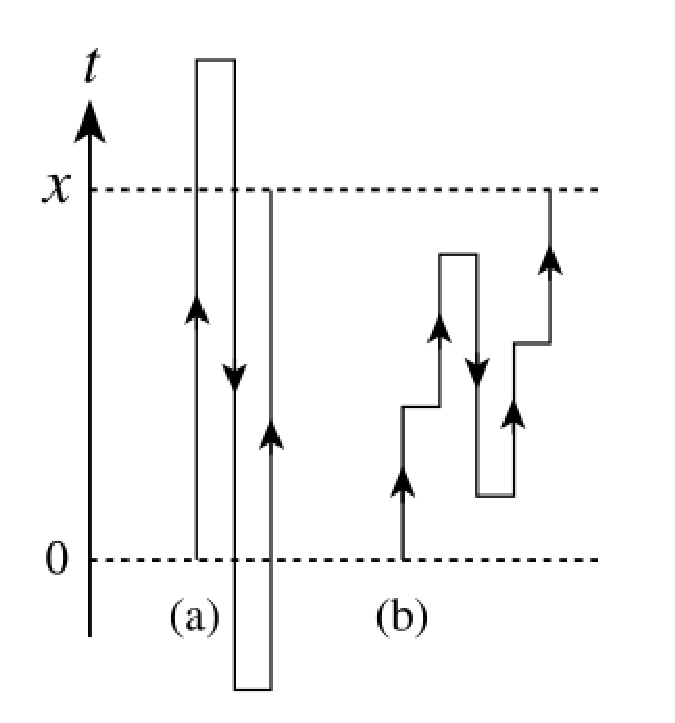
\includegraphics[width=5cm]{Plots/evolution.eps}
   \caption{Representation of the fourth-order approximation using (a) Eq.~\eqref{eq:fourth-order} and (b) Eq.~\eqref{eq:fourth-order-nopast}.} \label{plot:evolution}
\end{figure}


Now we can move to the sixth-order approximant, using $S_4(x)$ and following the same structure:
\begin{equation} \label{eq:sixth-order}
S_6(x) = S_4(s_4x)^2 S_4((1-4s_4)x) S_4(s_4x)^2,
\end{equation}
obtaining
\begin{equation}
4s_4^5 + (1-4s_4)^5 = 0 \quad \mathrm{or} \quad s_4 = \frac{1}{4-\sqrt[5]{4}} = 0.373065\ldots .
\end{equation}
We can continue this recursive procedure, ending up with the exact time evolution. It is easy to see that the procedure can be generalized with the following formula:
\begin{equation}
S_{2n+2} = S_{2n}(s_{2n}x)^2 S_{2n}((1-4s_{2n})x) S_{2n}(s_{2n}x)^2,
\end{equation}
where $s_{2n} = 1/(4-4^{\frac{1}{2n+1}})$.
It is interesting to note that the recursive procedure creates a fractal pattern composed by back-and-forth evolution, reproducing the exact time evolution.
\begin{figure}
  \centering
   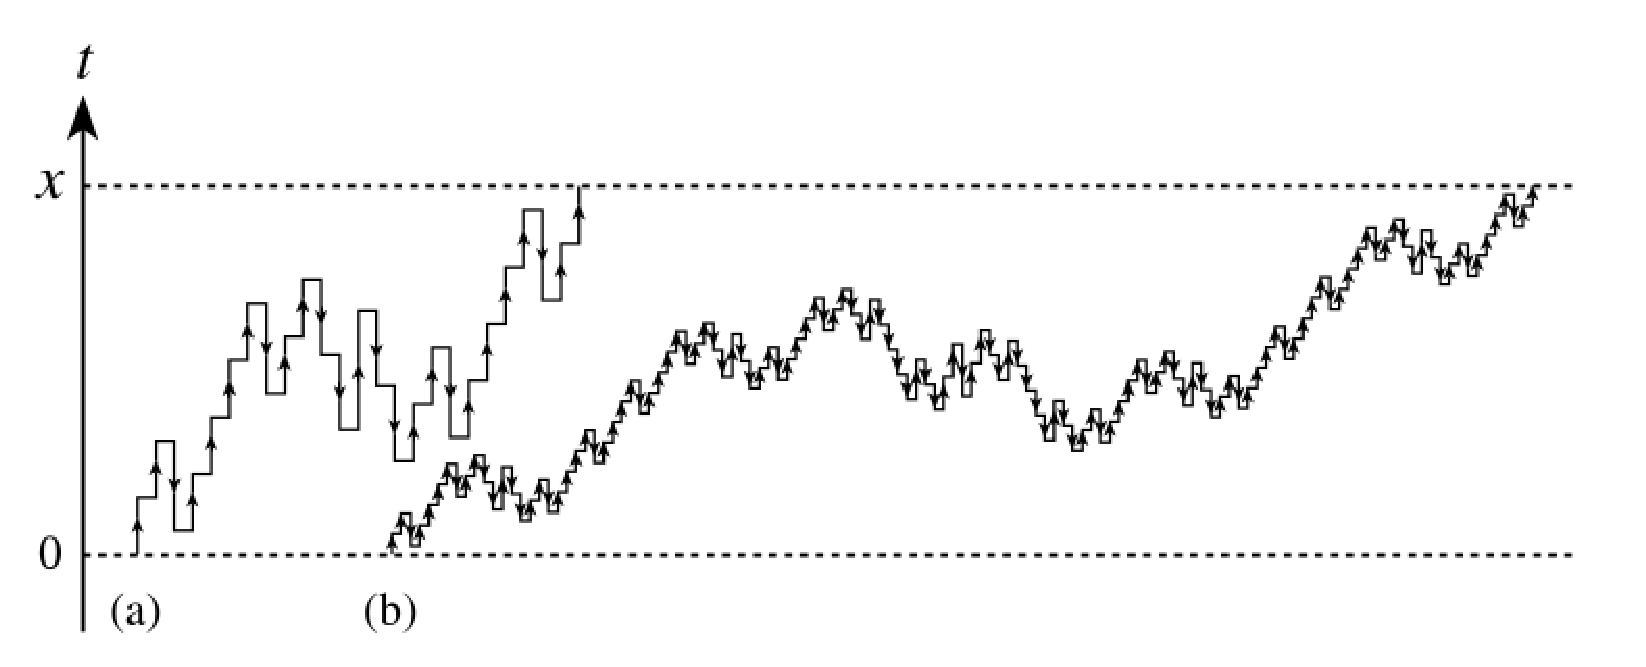
\includegraphics[width=8cm]{Plots/fractal_evolution.eps}
   \caption{Representation of the time evolution using (a) sixth-order approximant and (b) eighth-order approximant.} \label{plot:fractal-evolution}
\end{figure}

%%%%%%%%%%%%%%%%%%%%%%%%%%%%%%%%%%%%%%%%%%%%%%%%%%%%%%%%%%%%%%%%%%%%%%%%%%%%%%%
\section{Example: Spin Precession}
It is worthwhile to give a brief and simple example to show some remarkable properties of the Trotter--Suzuki decomposition. In this section, we compare it with the first order perturbation, using a simple example of quantum dynamics, namely, the spin precession.

\begin{figure}[t]
  \centering
   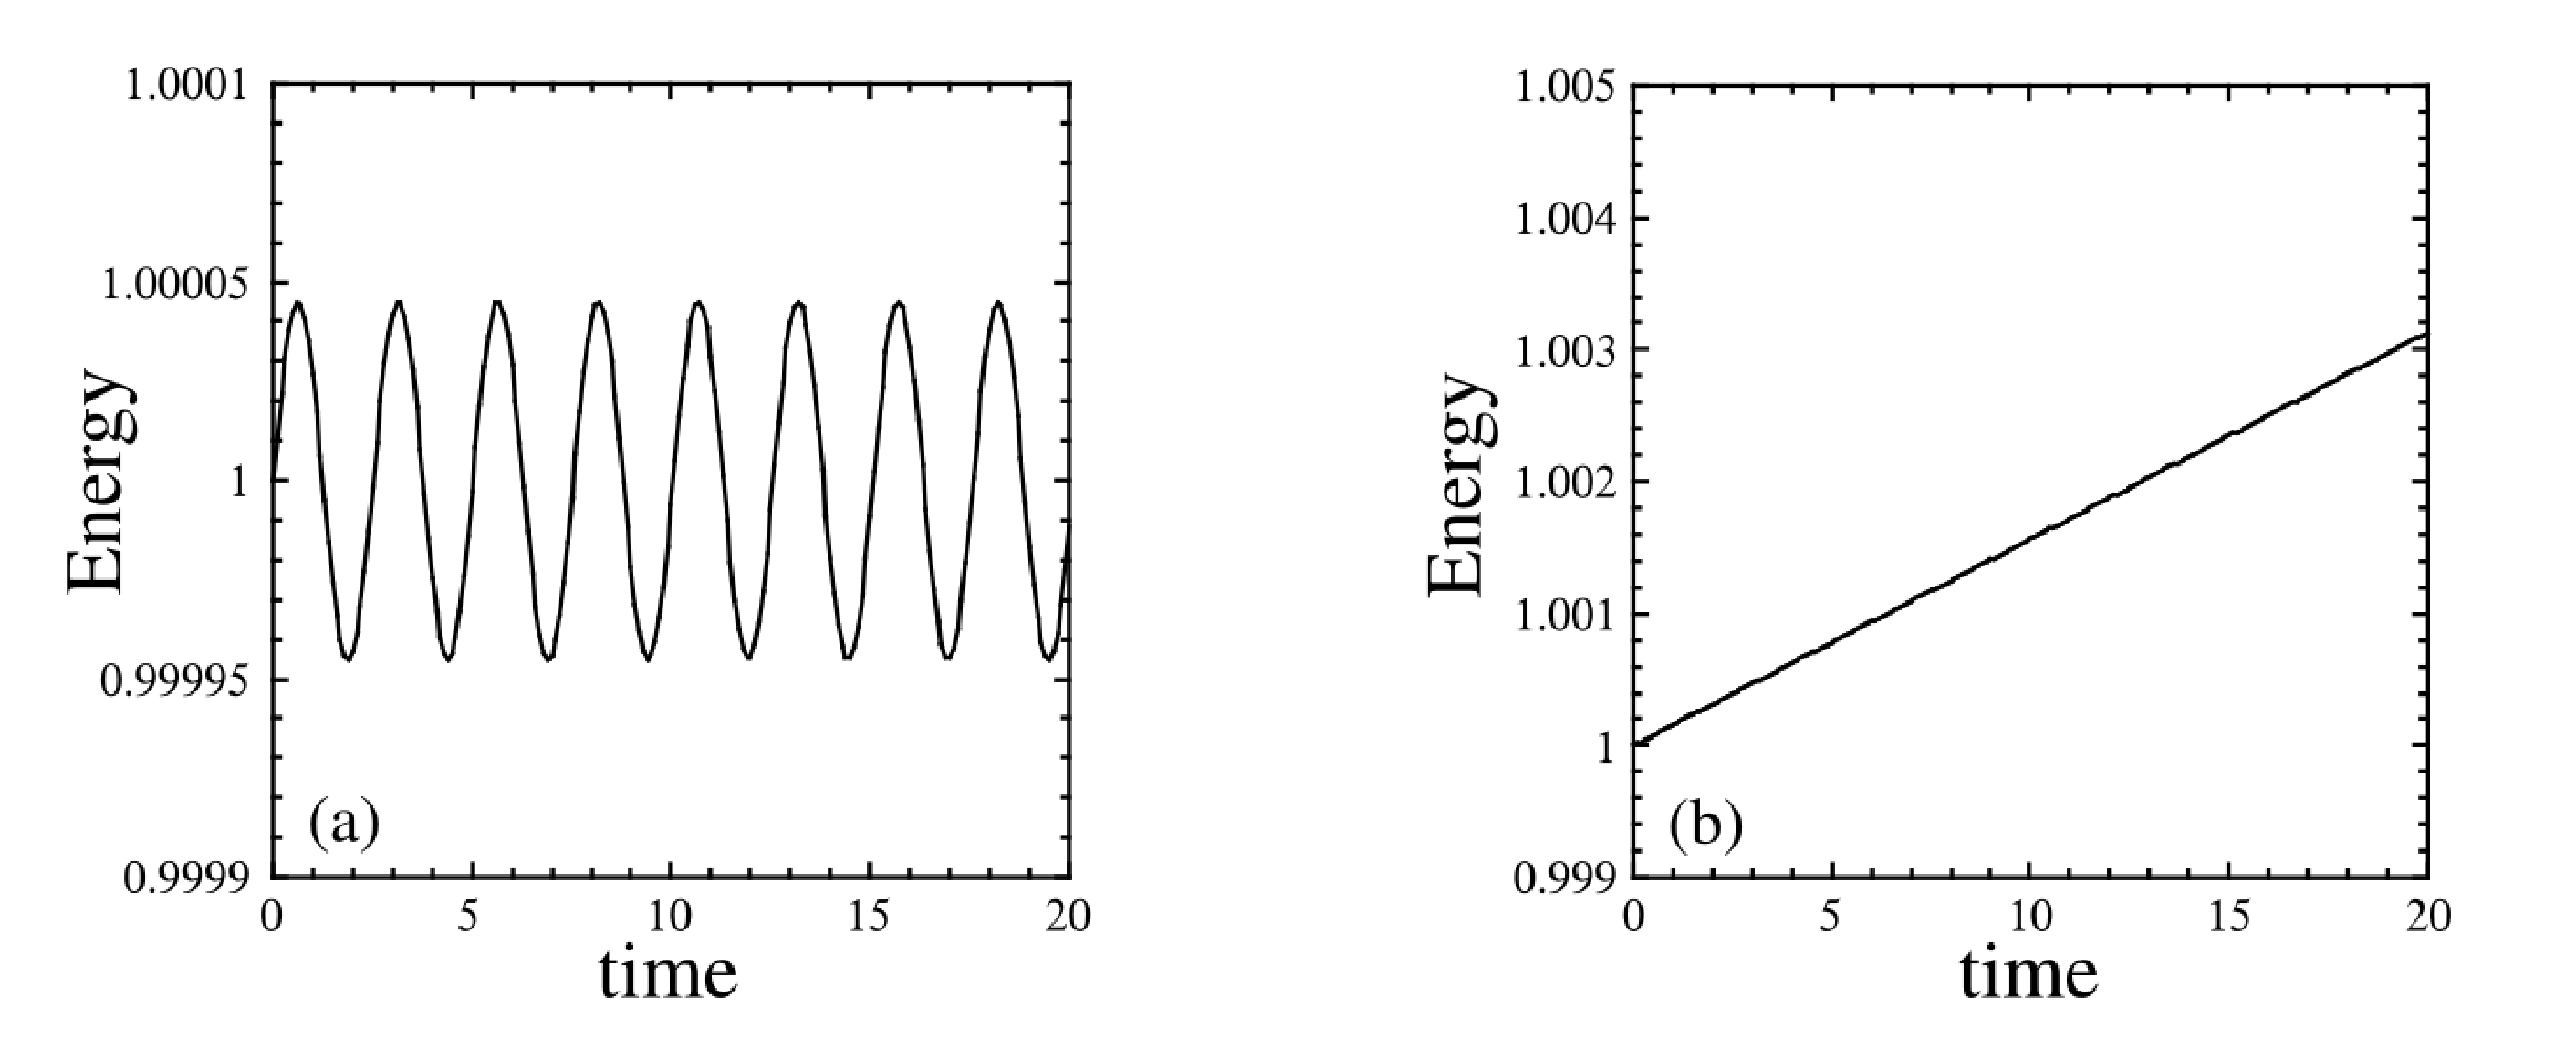
\includegraphics[width=12cm]{Plots/spin_evolution.eps}
   \caption{Energy expectation value for (a) the Trotter--Suzuki approximation~\eqref{eq:trotter-approximant} and (b) the perturbation approximation~\eqref{eq:perturbational-approximant}.} \label{plot:spin-evolution}
\end{figure}

Consider the following Hamiltonian:
\begin{equation}
H = \sigma_z + \Gamma \sigma_x,
\end{equation}
where $\Gamma$ is a real number, and, as initial state, the up-spin state
\begin{equation}
\psi(0) = 
\begin{pmatrix}
1 \\ 0
\end{pmatrix}.
\end{equation}
The evolution is simple to calculate analytically: the spin precesses around the axis of the magnetic field $\vec{H} = (\Gamma, 0, 1)$ with the period
\begin{equation}
T = \frac{\pi}{\sqrt{1+\Gamma^2}}.
\end{equation}
\begin{comment}
In the basis of the eigenvector of $\sigma_z$, the evolution operator is:
\begin{equation}
U(t) = \exp \left( -\frac{\imath t}{\hbar} H \right) = \exp \left( -\frac{\imath t}{\hbar} \right) \begin{pmatrix}
\cos \left( \frac{\Gamma t}{\hbar} \right) & \imath \sin \left( \frac{\Gamma t}{\hbar} \right) \\
\imath \sin \left( \frac{\Gamma t}{\hbar} \right) & \cos \left( \frac{\Gamma t}{\hbar} \right) \\
\end{pmatrix}
\end{equation}
\end{comment} 
However, here we use the Trotter approximation
\begin{equation} \label{eq:trotter-approximant}
\exp\left({-\frac{\imath}{\hbar}H \delta t}\right) = \exp\left({-\frac{\imath}{\hbar} \sigma_z \delta t}\right) \exp\left({-\frac{\imath}{\hbar} \Gamma \sigma_x \delta t}\right),
\end{equation}
and the perturbational approximant
\begin{equation} \label{eq:perturbational-approximant}
\exp\left({-\frac{\imath}{\hbar}H \delta t}\right) = I - \frac{\imath}{\hbar}(\sigma_z + \Gamma\sigma_x) \delta t,
\end{equation}
Due to the approximations used, the energy expectation $\langle H \rangle$ is not constant throughout the evolution Fig.~\ref{plot:spin-evolution}(a), as we would expect in the exact solution. However, with the Trotter approximation, the error in the energy expectation oscillates periodically, and never increases beyond the oscillation amplitude. This behavior is consistent with the property of the approximation: due to the unitarity, the state periodically comes back to the initial state with a good accuracy, producing the oscillation pattern in the energy.


In contrast, the error in the energy monotonically grows in the case of the perturbational approximant, as is shown in Fig.~\ref{plot:spin-evolution}(b). Indeed, with this approximation, the norm of the wave vector increases by the factor
\begin{equation}
\Vert 1 - \frac{\imath}{\hbar} H \Delta t H \Vert \simeq 1 + \Delta t \Vert H \Vert > 1.
\end{equation}

This simple example shows how the unitarity of the Trotter approximation improves the quality of the simulation, compared to the perturbation approximation.

%%%%%%%%%%%%%%%%%%%%%%%%%%%%%%%%%%%%%%%%%%%%%%%%%%%%%%%%%%%%%%%%%%%%%%%%%%%%%%%%%%%%
\section{Example: Symplectic Integrator}
Another interesting example regards the study of chaotic dynamics. In this case it is important to keep the symplecticity of the Hamilton dynamics.

Consider a classical Hamiltonian
\begin{equation}
H(\vec{p}, \vec{q}) = K(\vec{p}) + V(\vec{q}),
\end{equation}
where $K(\vec{p})$ is the kinetic term and $V(\vec{q})$ the potential term. The Hamilton equation is expressed in the form
\begin{equation}
\frac{\mathrm{d}}{\mathrm{d} t} 
\left( \begin{matrix}
\vec{p}(t) \\
\vec{q}(t)
\end{matrix} \right)
= 
\left( \begin{matrix}
- \frac{\mathrm{d}}{\mathrm{d} \vec{q}} V(\vec{q}) \\
\frac{\mathrm{d}}{\mathrm{d} \vec{p}} K(\vec{p})
\end{matrix} \right)
\equiv
\left( \begin{matrix}
 & - \hat{V} \cdot \\
\hat{K} \cdot &
\end{matrix} \right)
\left( \begin{matrix}
\vec{p} \\
\vec{q}
\end{matrix} \right)
\end{equation}
where the operators $\hat{K} \cdot$ and $\hat{V} \cdot$ act in the following way
\begin{equation}
\hat{K} \cdot \vec{p} \equiv \frac{\mathrm{d}}{\mathrm{d} \vec{p}} K(\vec{p}) \quad \mathrm{and} \quad \hat{V} \cdot \vec{q} \equiv \frac{\mathrm{d}}{\mathrm{d} \vec{q}} V(\vec{q}).
\end{equation}
We can define the "Hamiltonian" operator as $\mathcal{H} = \mathcal{K} + \mathcal{V}$ with
\begin{equation}
\mathcal{K} \equiv \left( \begin{matrix}
 &  \\
\hat{K} \cdot &
\end{matrix} \right)
\quad \mathrm{and} \quad
\mathcal{V} \equiv \left( \begin{matrix}
 &  -\hat{V} \cdot \\
 &
\end{matrix} \right)
\end{equation}
The two operators, $\mathcal{K}$ and $\mathcal{V}$, do not commute. This make the exponential of $\mathcal{H}$ not easily tractable. However, the exponential of  $\mathcal{K}$ and $\mathcal{V}$ is easier to calculate.

We notice that $\mathcal{K}^2 = \mathcal{V}^2 = 0$, and therefore we have
\begin{align}
\exp \left( \mathcal{K} \Delta t \right) \left( \begin{matrix}
\vec{p} \\ \vec{q}
\end{matrix} \right)
&=
(I+\mathcal{K}\Delta t) \left( \begin{matrix}
\vec{p} \\ \vec{q}
\end{matrix} \right)
=
\left( \begin{matrix}
\vec{p} \\ \vec{q} + \Delta t \frac{\mathrm{d}}{\mathrm{d} \vec{p}} K(\vec{p})
\end{matrix} \right), \\
\exp \left( \mathcal{V} \Delta t \right) \left( \begin{matrix}
\vec{p} \\ \vec{q}
\end{matrix} \right)
&= (I+\mathcal{V}\Delta t) \left( \begin{matrix}
\vec{p} \\ \vec{q}
\end{matrix} \right)
=
\left( \begin{matrix}
\vec{p} - \Delta t \frac{\mathrm{d}}{\mathrm{d} \vec{q}} V(\vec{q}) \\ \vec{q} 
\end{matrix} \right).
\end{align}
Thus, given the form of $K(\vec{p})$ and $V(\vec{q})$ the Trotter approximation of the evolution operator is determined.

Umeno and Suzuki~\citep{US93,SU93} demonstrated the use of symplectic integrators for chaotic dynamics of the system
\begin{equation}
K(\vec{p}) = \frac{1}{2} (p_1^2 + p_2^2) \quad \mathrm{and} \quad V(\vec{q}) = \frac{1}{2} 	q_1^2 q_2^2.
\end{equation}
The dynamic is constrained by the constant $\frac{\mathrm{d}}{\mathrm{d} t} |q_1(t) q_2(t)| = 0$, thus tuple $(q_1(t), q_2(t))$ is confined in the area surrounded by four hyperbolas as illustrated in Fig.~\ref{plot:configuration-space}. The Trotter approximation of the dynamics, gives  the energy fluctuation shown in Fig.~\ref{plot:Energy-trotter-chaotic}. Although the energy deviates from the correct value sometimes, it comes back after the deviation. The major deviations occur when the system goes into one of the four narrow valleys of the potential, while they are suppressed when the system is in the central area.

Contrary to this behaviour, the perturbation approximation
\begin{equation}
\left( \begin{matrix}
\vec{p} \\ \vec{q}
\end{matrix} \right) \longrightarrow (I + \Delta t \mathcal{H})
\left( \begin{matrix}
\vec{p} \\ \vec{q}
\end{matrix} \right)
=
\left( \begin{matrix}
\vec{p} - \Delta t \frac{\mathrm{d}}{\mathrm{d} \vec{q}} V(\vec{q}) \\ 
\vec{q} + \Delta t \frac{\mathrm{d}}{\mathrm{d} \vec{p}} K(\vec{p})
\end{matrix} \right),
\end{equation}
yields the monotonic energy increase shown in Fig.~\ref{plot:Energy-perturb-chaotic}. The reason of the difference between the approximants must be keeping the symplecticity, or the conservation of the phase-space volume.
\begin{figure}[t]
\centering
\begin{tabular}{ccc}
\subfloat[]{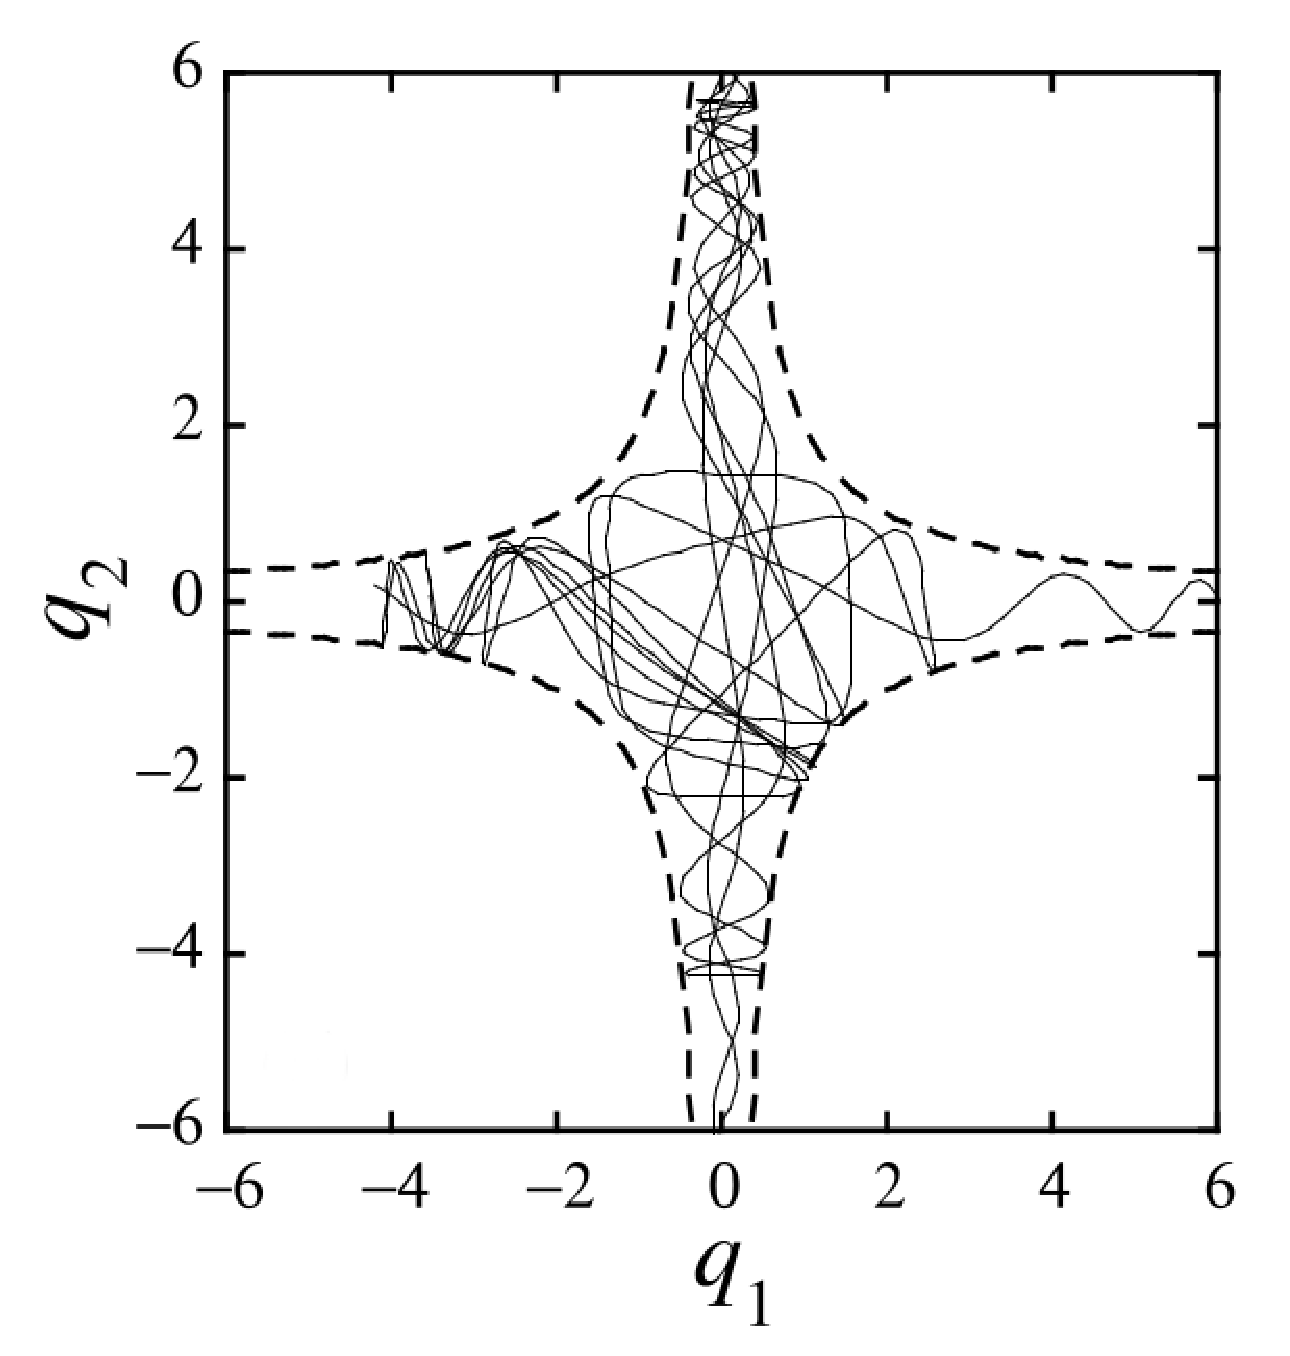
\includegraphics[width=3.7cm]{Plots/configuration-space.eps} \label{plot:configuration-space}} & 
\subfloat[]{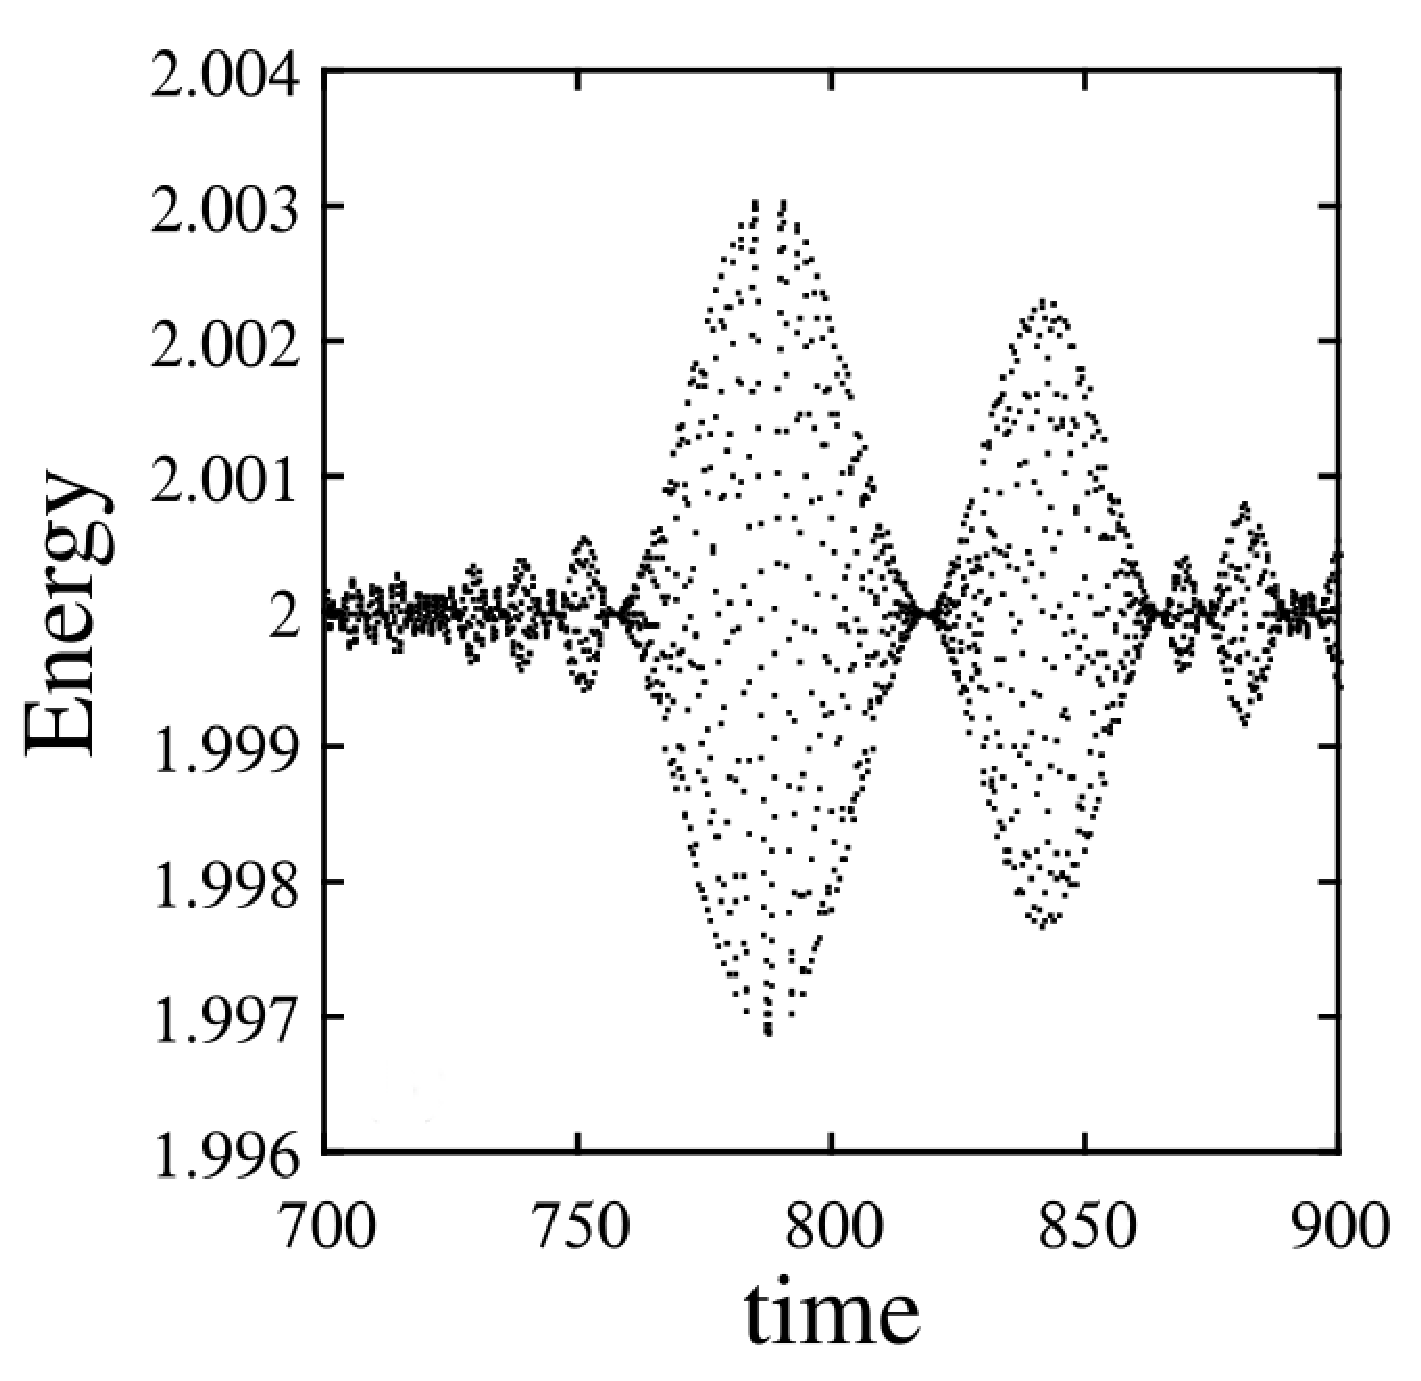
\includegraphics[width=4cm]{Plots/Energy-Trotter-Chaotic.eps} \label{plot:Energy-trotter-chaotic}} & 
\subfloat[]{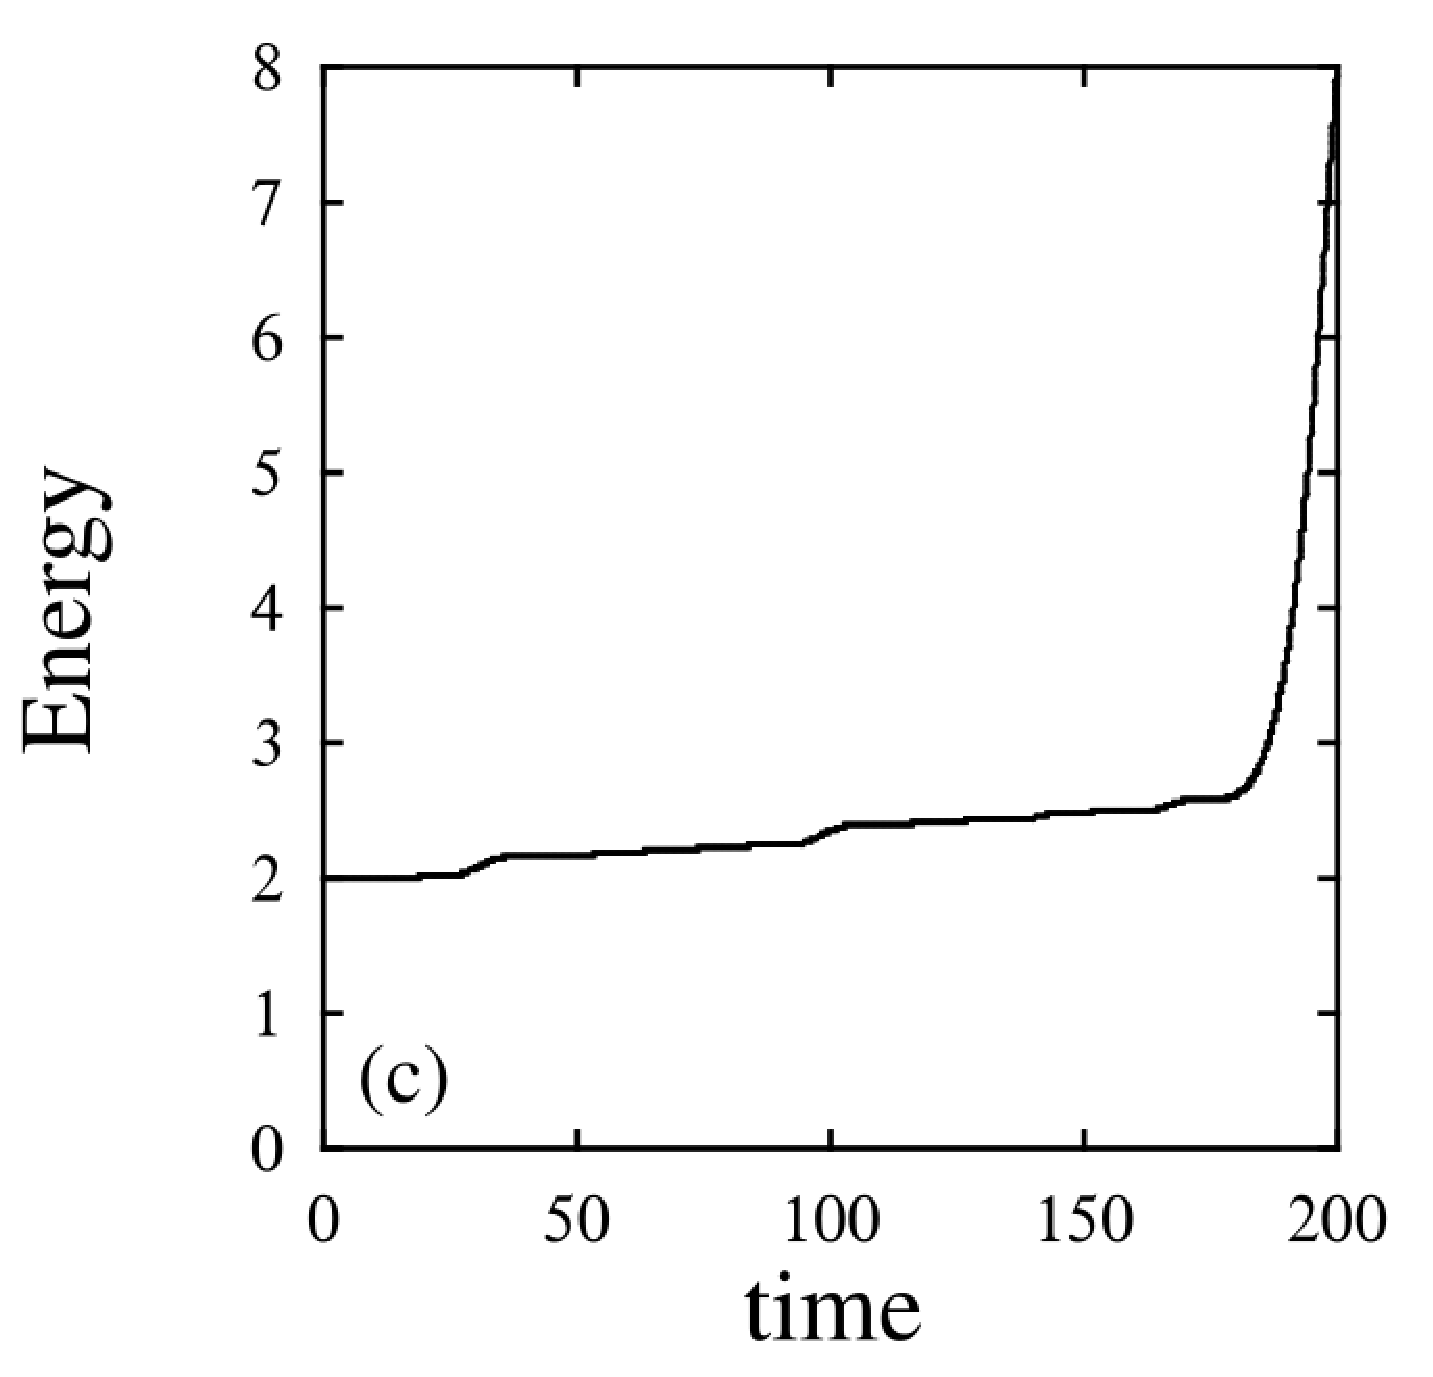
\includegraphics[width=4cm]{Plots/Energy-Perturbation-Chaotic.eps} \label{plot:Energy-perturb-chaotic}} \\
\end{tabular}
\caption{Evolution of the point in the configuration space, using the Trotter approximation. The initial condition is $p_1 = p_2 = 0$ and $q_1 = 2$, $q_2 = 1$~\ref{plot:configuration-space}. The energy fluctuation due to the Trotter approximation~\ref{plot:Energy-trotter-chaotic}. The energy increase due to the perturbation approximation~\ref{plot:Energy-perturb-chaotic}} \label{plot:Chaotic-system}
\end{figure}

\chapter{Decomposition of Unitary Evolution}
When it comes to solving differential equations that determine the behaviour of a physical system, an accurate approximation is often needed to find an explicit solution. As we have seen in the previous chapter, a good approach is to use the Trotter--Suzuki approximation. 

In this chapter we are interested in calculating the evolution operator $U(t) = \exp \left( - \frac{\imath t}{\hbar} H \right)$, the solution of the time-dependent Schr\"odinger equation, using the second order Trotter--Suzuki approximation. The Trotter--Suzuki approximation is based on the splitting of the exponent in a sum of operators. Thus, starting from a exponential that is difficult to calculate, we end up with a product of easy-to-calculate exponentials. In the next sections, we discuss how to decompose the Hamiltonian and the eventual calculation of the exponential.

%%%%%%%%%%%%%%%%%%%%%%%%%%%%%%%%%%%%%%%%%%%%%%%%%%%%%%%%%%%%%%%%%%%%%%%%
\section{Hamiltonian Decomposition}
We consider a single quantum particle in two dimensions in time-independent potential. The Hamiltonian operator of such system is written as follows
\begin{equation} \label{eq:hamiltonian-implementation}
\hat{H} = \frac{\hat{P}_x^2 + \hat{P}_y^2}{2m} + \hat{V},
\end{equation}
where $m$ is the particle mass and $\hat{V}$ is the external potential.

We use the coordinate reppresentation of the operators, so the kinetic term becomes
\begin{subequations}
\begin{align}
\bra{x,y} \frac{1}{2m} \left( P_x^2 + P_y^2 \right) \ket{\psi} = & \int \mathrm{d}x' \mathrm{d}y' \bra{x,y} \left( P_x^2 + P_y^2 \right) \ket{x',y'} \braket{x',y'|\psi} \label{eq:tot-momentum1} \\
= & - \frac{\hbar^2}{2m} \left( \nabla_x^2 + \nabla_y^2 \right) \psi(x,y) \label{eq:tot_momentum}
\end{align}
\end{subequations}
In this basis, the exponentiation of the external potential operator is straightforward, since it is diagonal. On the contrary, this is not true for the kinetic operator.

We consider the discretization of the continuum space into a uniform mesh, where $\Delta$ is the distance between any two consecutive points. We use the tuple $(i,j)$ to label the points of the mesh, with $i,j = 1,\ldots , N$, so that $\psi(x,y) \rightarrow \psi_{i,j}$ and $\ket{x,y} \rightarrow \ket{i,j}$. Using the second-order derivative central difference, we have:
\begin{equation} \label{eq:second-order-derivative}
\frac{\partial^2 \psi}{\partial x^2} \bigg|_{i,j} = \frac{\psi(i+1,j) - 2 \psi(i,j) + \psi(i-1,j)}{\Delta^2} + O(\Delta^2),
\end{equation}
Then we can write the Eq.~\eqref{eq:tot_momentum} as
\begin{equation} \label{eq:discr-tot-momentum}
\bra{i,j} \frac{1}{2m} \left( P_x^2 + P_y^2 \right) \ket{\psi} = -\frac{\hbar^2}{2m\Delta^2} \left( \psi_{i+1,j} + \psi_{i,j+1} + \psi_{i-1,j} + \psi_{i,j-1} - 4 \psi_{i,j} \right).
\end{equation}
To explicitly determine the matrix elements of the kinetic operator, let us rewrite the Eq.~\eqref{eq:discr-tot-momentum} using Kroneker's delta
\begin{align} \label{eq:delta-k-momentum}
\bra{i,j} \frac{1}{2m} \left( P_x^2 + P_y^2 \right) \ket{\psi} = & \sum_{k,l} -\frac{\hbar^2}{2m\Delta^2} [ \left(  \delta_{i+1,k} + \delta_{i-1,k} \right) \delta_{j,l} \, +  \\ 
+ &  \left( \delta_{j+1,l} + \delta_{j-1,l} \right) \delta_{i,k} - 4 \delta_{i,k} \delta_{j,l} ] \psi_{k,l}. \nonumber
\end{align}
Since the discretization of Eq.~\eqref{eq:tot-momentum1} led to the following equation
\begin{subequations}
\begin{align}
\bra{i,j} \frac{1}{2m} \left( P_x^2 + P_y^2 \right) \ket{\psi} = & \frac{1}{2m} \sum_{k,l} \bra{i,j} \left( P_x^2 + P_y^2 \right) \ket{k,l} \braket{k,l|\psi} \\
= & \frac{1}{2m} \sum_{k,l} \bra{i,j} \left( P_x^2 + P_y^2 \right) \ket{k,l} \psi_{k,l} \label{eq:discr-momentum}
\end{align}
\end{subequations}
from the comparison of Eq.~\eqref{eq:delta-k-momentum} and Eq.~\eqref{eq:discr-momentum}, we get
\begin{align} \label{eq:delta-kroneker}
\bra{i,j} \frac{1}{2m} \left( P_x^2 + P_y^2 \right) \ket{k,l} = -\frac{\hbar^2}{2m\Delta^2} & [ \left( \delta_{i+1,k} + \delta_{i-1,k} \right) \delta_{j,l} \, + \\ + & \left( \delta_{j+1,l} + \delta_{j-1,l} \right) \delta_{i,k} - 4 \delta_{i,k} \delta_{j,l} ]. \nonumber
\end{align}

We introduce two operators that will let us split the Hamiltonian into a sum of operators that are easy to exponentiate. We define:
\begin{equation} \label{eq:A-form}
A_{i,k} = \begin{cases} \delta_{i+1,k}, & \mbox{if } k\mbox{ is odd} \\ \delta_{i-1,k}, & \mbox{if } k\mbox{ is even} \end{cases}
\end{equation}
and
\begin{equation} \label{eq:B-form}
B_{j,l} = \begin{cases} \delta_{j-1,l}, & \mbox{if } l\mbox{ is odd} \\ \delta_{j+1,l}, & \mbox{if } l\mbox{ is even} \end{cases}
\end{equation}
Represented as matrices, these operators have the form of block diagonal matrices, namely:
\begin{equation}
A = \begin{pmatrix}
0 & 1 \\
1 & 0 \\
 & & 0 & 1 \\
 & & 1 & 0 \\
 & & & & 0 & 1 \\
 & & & & 1 & 0 \\
 & & & &  & & \ddots \\
\end{pmatrix}
\quad B = \begin{pmatrix}
0 \\
& 0 & 1 \\
& 1 & 0 \\
& & & 0 & 1 \\
& & & 1 & 0 \\
& & & & & 0 & 1 \\
& & & & & 1 & 0 \\
& & & & &  & & \ddots \\
\end{pmatrix}
\end{equation}
Using the new operators we can rewrite Eq.~\eqref{eq:delta-kroneker} as follow
\begin{align}
\bra{i,j} \frac{1}{2m} \left( P_x^2 + P_y^2 \right) \ket{k,l} = -\frac{\hbar^2}{2m\Delta^2}  [ & \left( A_{i,k} + B_{i,k} \right) \delta_{j,l} \, + \\ + & \left( A_{j,l} + B_{j,l} \right) \delta_{i,k} - 4 \delta_{i,k} \delta_{j,l} ] \nonumber
\end{align}
For the brevity of notation, we adopt the operator notation, so that the previous equation becomes
\begin{equation} \label{eq:mom-decomposition}
\frac{1}{2m} \left( \hat{P}_x^2 + \hat{P}_y^2 \right)= -\frac{\hbar^2}{2m\Delta^2} \left[ \hat{A}_x + \hat{B}_x + \hat{A}_y + \hat{B}_y - 4 \hat{I} \right],
\end{equation}
where the label indicates the index to which the operator acts, so that the following commutation rules are satisfied:
\begin{equation}
[\hat{A}_x, \hat{A}_y] = 0 \quad [\hat{A}_x, \hat{B}_y] = 0 \quad [\hat{B}_x, \hat{A}_y] = 0 \quad [\hat{B}_x, \hat{B}_y] = 0.
\end{equation} 
Finally, by mean of Eq.~\eqref{eq:mom-decomposition}, we get the decomposition formula for the Hamiltonian~\eqref{eq:hamiltonian-implementation}:
\begin{equation} \label{eq:hamiltonian-decomposition}
\hat{H} = -\frac{\hbar^2}{2 m \Delta^2} \left[ \hat{A}_x + \hat{B}_x + \hat{A}_y + \hat{B}_y - 4 \hat{I} \right] + \hat{V}.
\end{equation}

%%%%%%%%%%%%%%%%%%%%%%%%%%%%%%%%%%%%%%%%%%%%%%%%%%%%%%%%%%%%%%%%%%%%%%%%%%%%%%%%%%%%%%%%%
\section{Evolution Operator}
In the previous section, we shown how to split the Hamiltonian in the discrete space approximation. Now we explicitly calculate the Trotter--Suzuki decomposition for the evolution operator. Using the Hamiltonian decomposition~\eqref{eq:hamiltonian-decomposition}, the evolution operator $\hat{U}(t) = \exp(-\frac{\imath t}{\hbar} H)$ can be written as follows, in the first Trotter--Suzuki approximation
\begin{align} \label{eq:1approxTS}
\hat{U}_1(t) = \exp\left(-\frac{\imath t}{\hbar}\left(\hat{V} + \frac{2 \hbar^2}{m \Delta^2} \hat{I}\right) \right) & \exp\left(\imath \alpha \hat{A}_x \right) \exp\left(\imath \alpha \hat{B}_x \right) \cdot \\ \cdot & \exp\left(\imath \alpha \hat{A}_y \right) \exp\left(\imath \alpha \hat{B}_y \right) + O(t^2) \nonumber
\end{align}
where we defined $\alpha = \frac{\hbar t}{2m\Delta^2}$. 

Using the equality 
\begin{equation}
\exp(\imath \alpha \sigma) = I \cos(\alpha) + \imath \sigma \sin(\alpha),
\end{equation}
it is straightforward to calculate the exponential of the operators $A$ and $B$, since they are diagonal matrices of the Pauli matrix:
\begin{equation} \label{eq:expA}
\exp\left(\imath \alpha \hat{A}_x \right) = \hat{I}_x \cos(\alpha) + \imath \sin(\alpha) \hat{A}_x
\end{equation}
\begin{equation} \label{eq:expB}
\exp\left(\imath \alpha \hat{B}_x \right) = \hat{I}_x (\cos(\alpha)(1-\delta_{x,0}) + \delta_{x,0}) + \imath \sin(\alpha) \hat{B}_x
\end{equation}
The first exponential in Eq.~\eqref{eq:1approxTS} is also straightforward to calculate. Indeed $\hat{V} \ket{i,j} = V(i,j) \ket{i,j}$ so,
\begin{equation}
\bra{k,l} \exp\left(-\frac{\imath t}{\hbar}\left(\hat{V} + \frac{2 \hbar^2}{m \Delta^2} \hat{I}\right) \right) \ket{i,j} = \delta_{k,i} \delta_{l,j} \exp\left( -\frac{\imath t}{\hbar} \left( V(i,j) + \frac{2 \hbar^2}{m \Delta^2} \right) \right)
\end{equation}
The second order approximation of Trotter--Suzuki decomposition is easily calculated using $U_1(t)$, namely
\begin{equation} \label{eq:second-TS-evo-operator}
\hat{U}_2(t) = \hat{U}_1\left( -\frac{t}{2} \right)^\dagger \hat{U}_1\left(\frac{t}{2}\right)
\end{equation}

%%%%%%%%%%%%%%%%%%%%%%%%%%%%%%%%%%%%%%%%%%%%%%%%%%%%%%%%%%%%%%%%%%%%%%%%%%%%%%%%%%%%%%%%%
\section{Evolution Towards the Ground-state}
A reliable and easily-implemented method of approximating the ground state of the
system is by propagation in imaginary time. Consider the Schr\"odinger equation
\begin{equation}
\imath \hbar \frac{\partial \ket{\psi(t)}}{\partial t} = \hat{H} \ket{\psi(t)}.
\end{equation}
The transformation $ \tau = \imath t$ lead to the equation
\begin{equation}
\hbar \frac{\partial \ket{\psi(\tau)}}{\partial \tau} = - \hat{H} \ket{\psi(\tau)}.
\end{equation}
The formal solution for this equation, with initial condition $\ket{\psi(0)} = \ket{\psi_0}$ is $\ket{\psi(\tau)} = \exp\left( -\frac{\tau}{\hbar} H \right) \ket{\psi_0}$. The initial state $\ket{\psi_0}$ can be written as a linear combination of Hamiltonian's eingenvectors:
\begin{equation}
\ket{\psi_0} = \sum_i c_i \ket{\phi_i},
\end{equation}
where $\hat{H} \ket{\phi_i} = E_i \phi_i$ for $i = 0,1,2,\ldots$~. In this basis $\ket{\psi(\tau)}$ can be written as follow
\begin{equation}
\ket{\psi(\tau)} = \sum_i c_i \exp\left( -\frac{\tau}{\hbar} E_i \right) \ket{\phi_i}.
\end{equation}
Taking $E_0$ as the ground-state energy, we can rearrange the previous equation
\begin{equation} \label{eq:imag-evolution}
\ket{\psi(\tau)} = \exp \left( -\frac{\tau}{\hbar} E_0 \right) \sum_i c_i  \exp\left( -\frac{\tau}{\hbar} \Delta E_i \right) \ket{\phi_i}.
\end{equation}
where $\Delta E_i = E_i - E_0 > 0,  \forall i > 0$. We now take the limit for $\tau \rightarrow +\infty$. As long as the initial state is not orthogonal to the ground state, namely $c_0 \neq 0$, the leading term in the sum of Eq.~\eqref{eq:imag-evolution} is given by the ground state
\begin{equation}
\lim_{\tau \rightarrow +\infty} \ket{\psi(\tau)} = \exp \left( -\frac{\tau}{\hbar} E_0 \right) c_0 \ket{\phi_0}.
\end{equation}
Thus, evolving the initial state for a sufficient amount of time, let us to reach an  approximation of the ground state.

We implement the evolution operator in imaginary time using the same Trotter--Suzuki decomposition and Hamiltonian splitting as for the real time evolution. The operator reads as
\begin{equation}
\hat{U}(\tau) =   \exp\left(-\frac{\tau}{\hbar} \left( -\frac{\hbar^2}{2 m \Delta^2} \left[ \hat{A}_x + \hat{B}_x + \hat{A}_y + \hat{B}_y - 4 \hat{I} \right] + \hat{V} \right) \right)
\end{equation} 
so in the first Trotter--Suzuki approximation we have
\begin{align}
\hat{U}_1(t) = \exp\left(-\frac{\tau}{\hbar}\left(\hat{V} + \frac{2 \hbar^2}{m \Delta^2} \hat{I}\right) \right) & \exp\left(\alpha_\tau \hat{A}_x \right) \exp\left( \alpha_\tau \hat{B}_x \right) \cdot \\ \cdot & \exp\left( \alpha_\tau \hat{A}_y \right) \exp\left( \alpha_\tau \hat{B}_y \right), \nonumber
\end{align}
where $\alpha_\tau = \frac{\hbar \tau}{2m\Delta^2}$. Using the equality
\begin{equation}
\exp( \alpha_\tau \sigma) = I \cosh(\alpha_\tau) +  \sigma \sinh(\alpha_\tau)
\end{equation}
we can calculate the exponential of $A$ and $B$ as
\begin{equation}
\exp\left( \alpha_\tau A_x \right) = I_x \cosh(\alpha_\tau) + \sinh(\alpha_\tau) A_x
\end{equation}
\begin{equation}
\exp\left( \alpha_\tau B_x \right) = I_x (\cosh(\alpha_\tau)(1-\delta_{x,0}) + \delta_{x,0}) +  \sinh(\alpha_\tau) B_x
\end{equation}
Finally, in the second order approximation we have:
\begin{equation}
\hat{U}_2(\tau) = \hat{U}_1\left( \frac{\tau}{2} \right)^\mathrm{T} \hat{U}_1\left(\frac{\tau}{2}\right)
\end{equation}



\chapter{Implementation}

%summarize on what we focused (NVA):
%-high performance
%-reliable
%-ease of use

In the previous chapter we have seen how we approximated the evolution operator. In the following we explain the algorithm that implements the problem.

Our main goal was to develop a high-performance algorithm. The algorithm uses a distribute version of highly optimized CPU and GPU kernels, that runs efficiently on a cluster. Particularly important for this purpose is the memory access pattern optimization. Large amount of data are stored in the main memory. These data need to be sent to the process unit to be processed. Nowadays, process units are by far faster in processing data than the ability of the main memories to fed them. So if the process unit had to fetch data from the main memory, it would be slowed to the velocity of the memory. To avoid this problem we exploit cache-aware computation that uses smaller and faster sub-system memories, dubbed caches. 
Furthermore, a distributed workload across a multiprocessor system requires a communication between the nodes. Indeed, to proceed to the next iteration, a node needs data of the previous iteration calculated by other nodes. The transfer of data in a network of nodes can be even slower than the transfer from main memory to process unit. However, in a certain extent, communication between nodes and calculation in process unit can be done in parallel. For the sake of efficiency, it is worth to overlap the two as much as possible.

For the purpose of developing reliable scientific software, we put emphasis on unit testing. In the development of complex software, it is important to test various part of the code, to be sure of its correctness. A program can be split into several units, each one having a define use and an expected behaviour. Based on this one develop a test to exercise the unit and verify its exactness. We exploit unit testing using the library CppUnit. Moreover, we use double-precision floating point operations, to gain accuracy in the simulations.

Our approach was also to ensure that our implementation fits in with rapid prototyping
systems. The program allows to the use of a command line interface, for the flexibility of the simulation. In addition, the function that performs the evolution is exposed as an application programming interface (API). We also developed wrappers to make the kernels accessible from Python and MATLAB.
%control version system

%kernel citation
Before entering in the details of the algorithm, we explain some concepts important for high performance code.

%%%%%%%%%%%%%%%%%%%%%%%%%%%%%%%%%%%%%%%%%%%%%%%%%%%%%%%%%%%%%%%%%%%%%%%%%%%%%%%%%%%%%%
\section{Cache optimization}
Nowadays there exist a large gap between CPU speed and main memory performance. To alleviate this gap, computer architectures implement hierarchical memory structures. This approach allows to work around both the low main memory bandwidth and the latency of main memory accesses.
The memory bandwidth is a measure of the rate at which data can be read from or stored into the memory by a processor, and it is a crucial parameter that affect an algorithm performance. Along with this factor also the memory latency play an important role in computer performance. The memory latency is the delay time between the moment a memory controller tells the memory module to access a particular memory location, and the moment these data are available on the module's output pins. These parameters characterized the velocity at which the memory can feed the processor. When the CPUs need to process a certain data it request it to the memory. Since that moment it will have to wait the time the date come up to the memory's output pins and the time they take to travel to the CPUs.
 
  The common structure of the hierarchy consist of a series of memories; the smaller they are, the closer they are to the CPUs; the cheaper they are, the further they are from the CPUs. Usually, at the top of the hierarchy there are the registers, memories integrated within the processor chip that can provide data with low latency and high bandwidth. Between the processor core and the main memory there are memories called \emph{cache memories} or \emph{caches}. Finally, there is the main memory, usually constituted of large and slow hard disk drives. During the execution of a program, some blocks of data are used more often than others, so the CPUs will work with this subset of data for most of the time. To get an efficient algorithm, the idea is to store frequently used blocks of data on fast memories: the more frequently the block is used, the higher in the hierarchy is the memory that stores it. 

Typically, the data residing within a smaller memory are also stored within the larger memory, so the levels of the memory hierarchy subset one another. A common memory hierarchy is show in Fig.~\ref{fig:memory-hierarchy}.
\begin{figure}
   \centering
   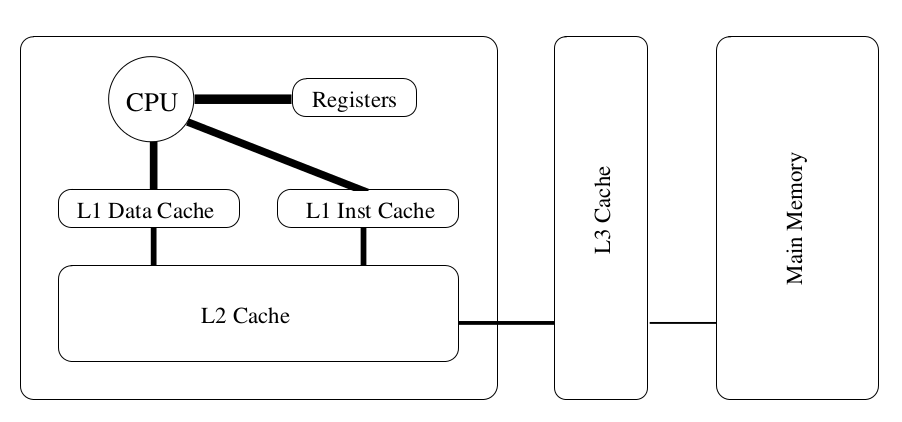
\includegraphics[width=10cm]{Figs/Memory_hierarchy.png}
   \caption{A Common memory hierarchy that present two on-chip L1 caches, on-chip L2 cache, and a third level of off-chip cache. The thickness of the interconnections illustrate the bandwidths between the memory hierarchy levels.} \label{fig:memory-hierarchy}
\end{figure} 

An efficient algorithm must be designed taking care of the memory hierarchical level. Unfortunately, compilers are not intended to introduce sophisticated cache-based transformations. Consequently, the optimization effort is left to the programmer. 

This aspect is particularly important when dealing with numerically intense codes, which occur in science and engineering disciplines, such as computational physics, mechanical engineering and computational fluid dynamic, just to cite some. These type of code are characterized by a large portion of floating-point (FP) operations. Thus, instruction cache misses do not significantly affect the execution performance. Much of the optimization effort concerns data access pattern. Indeed, due to data access latencies and memory bandwidth issues, it is not sufficient to optimize the number of arithmetic operation alone. Efficient codes in scientific computing must necessarily combine computationally optimal algorithms and memory hierarchy optimization.

%%%%%%%%%%%%%%%%%%%%%%%%%%%%%%%%%%%%%%%%%%%%%%%%%%%%%%%%%%%%%%%%%%%%%%%%%%%%%%%%%%%%
\subsection{Organization and Aspects of Cache Architectures}
The common memory hierarchy presents a rather small number of registers on the chip, which has almost no memory latency. On the chip we can also find a small cache -- usually called \textit{level one (L1) cache} -- limited to 64Kbyte, so that low latency and high bandwidth are assured. The latency of \textit{on-chip} caches is commonly one or two CPUs cycles. The L1 cache is often split into two separate parts; one only keeps data, the other instructions. The second level memory (L2) is tipically placed on-chip as well and it is usually limited to 1Mbyte. Due to the bigger size the  latency is around 5 to 10 cycles. Another cache level may be implemented off-chip if the L2 cache is on-chip. The L3 cache size may vary from 1MByte to 16MByte. They provide data with latency of about 10 to 20 cycles.

Data within the cache are stored in \textit{cache lines}. A cache line holds the contents of a contiguous block of main memory. We say that a \textit{cache hit} occur when the data requested by the processor are found in a cache line. If the data requested are not founded in the cache, a \textit{cache miss} occur. In the latter case, the contents of the \textit{memory block} containing the requested words are then fetched from a lower memory layer and copied into a cache line. This operation typically imply another data to be replaced by the new one requested, which is very inefficient. Indeed, the replacement of a cache line takes more time than the CPU to read the same date directly from the main memory. For this reason, caches implement strategy to increase the rate cache hits  over the cache misses. The optimal replacement strategy would be to replace the memory block which will not be accessed for the longest time. However, such strategy is impossible to implement since it requires information about future cache references. 

The most commonly used strategy is \textit{random} and \textit{least recently used (LRU)}. The former randomly chooses a cache line to be replaced. The latter replaces the block which has not been accessed for the longest time interval. Less common strategies are \textit{least frequently used (LFU)} and \textit{first in, first out (FIFO)}. The LFU replaces the memory block in the cache line which has least frequently been used, whereas the FIFO replaces the data which have been residing in cache for the longest time.

These strategy are based on the principle of \textit{locality} references~\cite{Hennessy-Patterson}, which states that recently used data are very likely to be reused in the near future. Locality can be of two different type: \textit{temporal} locality and \textit{spatial} locality. A sequence of references exhibits temporal locality if recently accessed data are likely to be accessed again in the near future. A sequence of references manifest spatial locality if data located close together in address space tend to be referred close together in time.

%%%%%%%%%%%%%%%%%%%%%%%%%%%%%%%%%%%%%%%%%%%%%%%%%%%%%%%%%%%%%%%%%%%%%%%%%%%%%%%%%%%%%%
\subsection{Data Access Optimizations}
The most straightforward and simple approach to implement an algorithm on a code, usually does not achieve the best execution performance. As we saw in the previous section, to reach this goal the programmer has to care about how the data are handled by the memory hierarchy and how the CPUs access to them. In scientific computation, this typically imply the need to apply transformation on the code, that change the order in which iterations in a loop nest are executed. Such transformations are part of \textit{data access optimizations} techniques, which goal is mainly to improve temporal locality. We present in this section data optimization techniques that preserve the final result.\footnote{Numerical results may slightly change due to the properties of finite precision arithmetic} We focus on a set of loop transformations that improve data locality for one level of the memory hierarchy: a cache.
\\

\noindent \textit{Loop Interchange}. This transformation reverse the order of two adjacent loops in a loop nest. This can be generalized to \textit{loop permutation} where more than two loops are moved at once.  %ref(2,65)

Loop interchange can improve locality by reducing the \textit{stride} of an array-based computation. The stride is the distance of array elements in memory accessed within consecutive loop iterations. For instance, suppose we want to calculate the square norm of a vector (Algorithm~\ref{algo:loop-interchange}). Furthermore suppose that the vector is stored in a (6,8) array in memory Fig.~\ref{fig:interchanged-loop-nests}, in \textit{row major order}; i.e. two array elements are stored adjacent in memory if their second indices are consecutive numbers. The code corresponding to the left part of Fig.~\ref{fig:interchanged-loop-nests}, accesses the array elements in a column-wise manner, so the stride is equal to 8. Consequently, the preloaded data in the cache line marked with grey color will not be reused if the array is too large to fit entirely in cache. The next data will be fetched from the main memory. Interchanging the loop nest allow the cache line to be reused, as the stride is now 1 (right part of Fig.~\ref{fig:interchanged-loop-nests}). \\
\begin{figure}
   \centering
   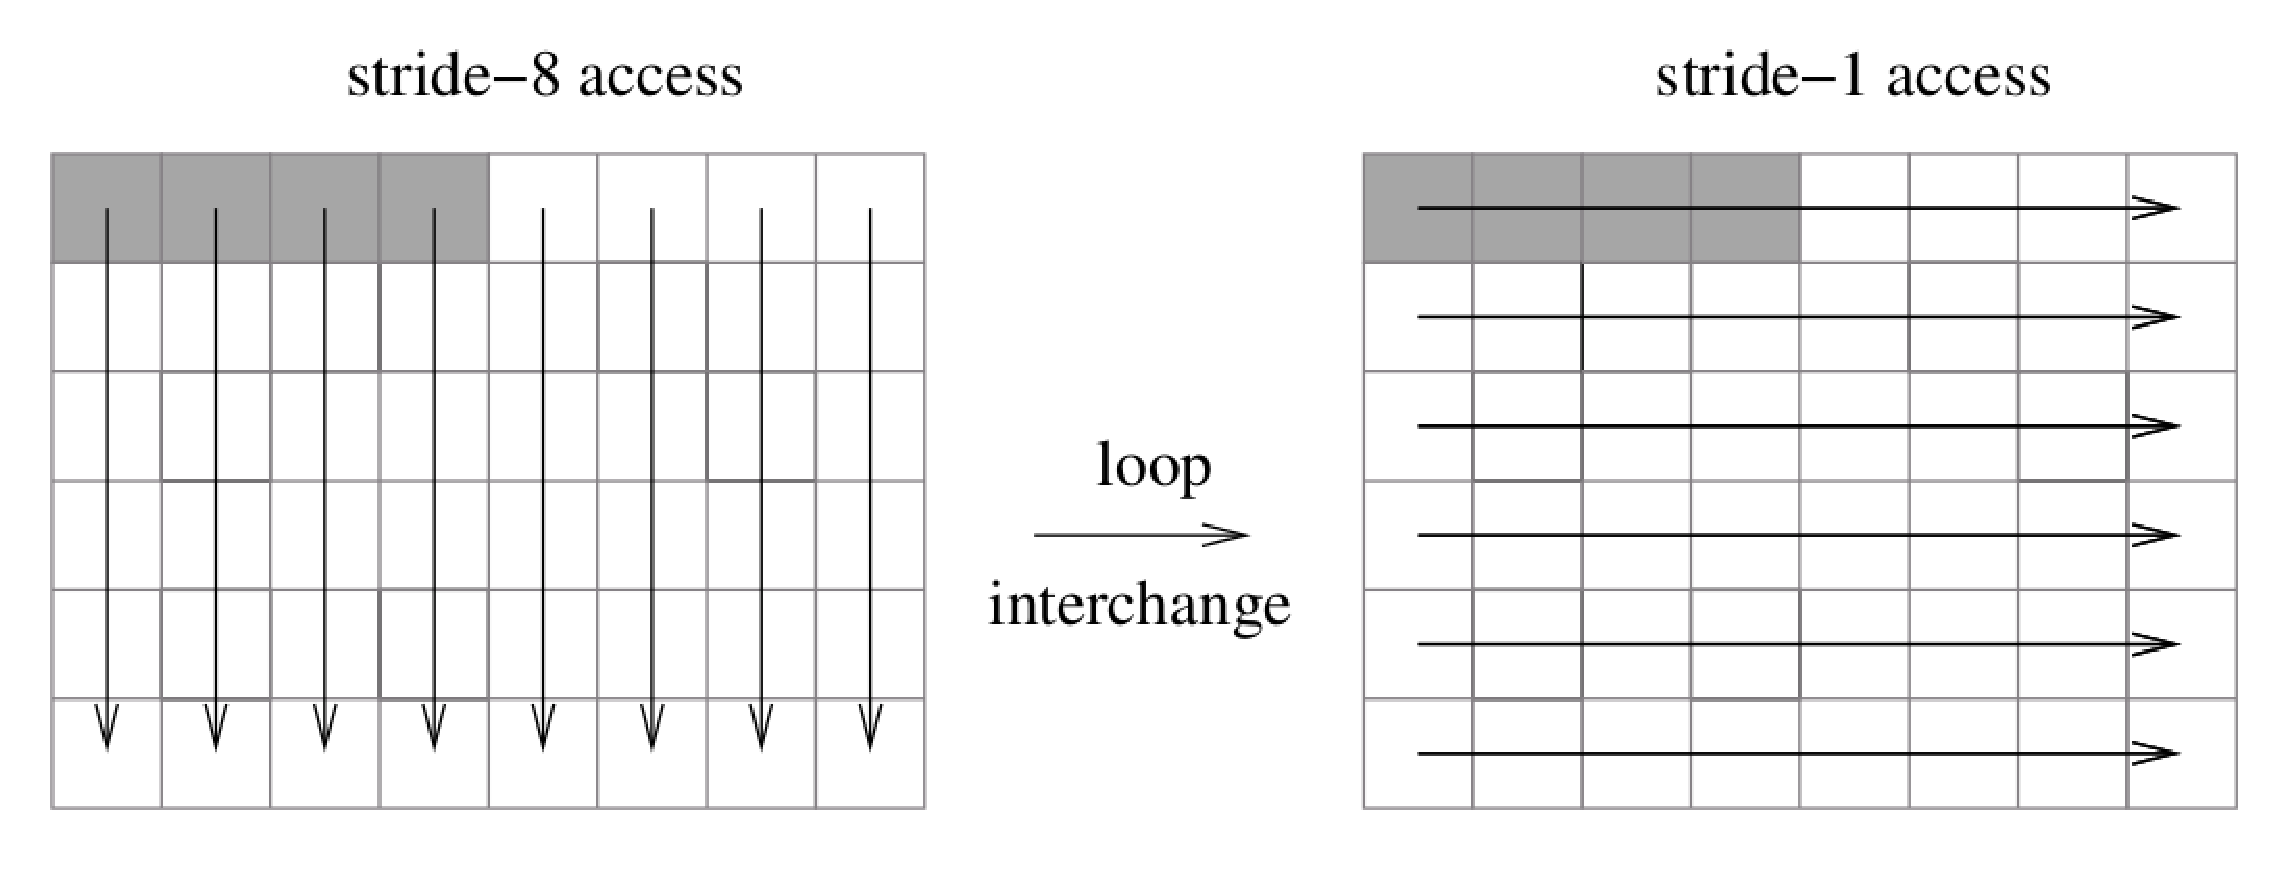
\includegraphics[width=10cm]{Figs/Interchanged_loop_nests.eps}
   \caption{Access pattern for interchenged loop nests in a (6,8) array.} \label{fig:interchanged-loop-nests}
\end{figure} 


\begin{algorithm}[t]
\SetAlgoLined
double $norm2$\;
double $a[n,n]$\;
//Original loop nest\;
\For{$j = 1$ \KwTo n }{
	\For{$i = 1$ \KwTo n }{
		$norm2 += a[i,j] \cdot a[i,j]$\;	
	}
}
\caption{Loop interchange} \label{algo:loop-interchange}
\end{algorithm}


\noindent \textit{Loop Fusion}. This transformation takes two adjacent loops that have the same iteration space traversal and combines their bodies into a single loop.%ref(17)
When Loop fusion can be applied -- when there are no instruction dependencies between the fused loops -- data locality may be improved. Assume that two consecutive loops perform global sweeps through an array as in the code shown in Algorithm~\ref{algo:loop-fusion},
and that the data are too large to fit entirely in the cache. When the first loop finish, the data of array \textit{b} are not completely loaded in cache, and the second loop will have to reload them from the main memory. If the two loops are combined with loop fusion only one global sweep through the array \textit{b} will be performed, resulting in less cache misses. \\
\begin{algorithm}[h]
//Original loop nest\;
\SetAlgoLined
\For{$i = 1$ \KwTo n }{
	$b[i] = a[i] + 1$\;
}
\For{$i = 1$ \KwTo n }{
	$c[i] = b[i] \cdot 3$\;
}
\caption{Loop fusion} \label{algo:loop-fusion}
\end{algorithm}

%\noindent \textit{Loop Blocking}. 

%%%%%%%%%%%%%%%%%%%%%%%%%%%%%%%%%%%%%%%%%%%%%%%%%%%%%%%%%%%%%%%%%%%%%%%%%%%%%%%%%%%%
\section{CPU kernels}
The code implements two CPU kernels: both are  cache optimized, but one is further optimized to use the SSE instruction set of the CPU. In this section we explain the CPU kernels in a single thread scenario and the cache optimization strategy adopted.

%%%%%%%%%%%%%%%%%%%%%%%%%%%%%%%%%%%%%%%%%%%%%%%%%%%%%%%%%%%%%%%%%%%%%%%%%%%%%%%%%%%%
\subsection{Matrix updating scheme}
The wave function of the system $\psi_{i,j}(0)$ is stored in two arrays in row major order, one for the real part and one for the imaginary part. The evolved wave function $\psi_{i,j}(t)$ is calculated dividing the time in small time intervals of length $\Delta t$. To have an accurate simulation, $\Delta t$ must satisfy the inequality $\Delta t \ll \frac{m \Delta L^2}{\hbar}$, where $m$ is the particle mass and $\Delta L$ is the distance between two consecutive dots of the mesh. Indeed if we exploit the Tailor expansion of the evolution operator
\begin{equation}
\mathrm{e}^{\frac{\imath}{\hbar}H\Delta t} = 1 + \frac{\imath}{\hbar}H\Delta t + O(\Delta t^2),
\end{equation} 
we have $1 \gg \frac{\Delta t}{\hbar}\parallel H \parallel $. Supposing that the leading term in the Hamiltonian is the kinetic term, the second-order derivative approximation (Eq.~\eqref{eq:second-order-derivative}) lead to $1 \gg \frac{\hbar}{m \Delta L^2} \Delta t$.

In the second-order Trotter-Suzuki approximation, the $\psi_{i,j}(\Delta t)$ is the result of nine matrix-vector products. From Eq.~\eqref{eq:second-TS-evo-operator} and Eq.~\eqref{eq:1approxTS}, we have
\begin{align} \label{eq:single-iteration}
\psi(\Delta t) = \mathrm{e}^{\imath \frac{\alpha}{2} \hat{A}_y} \mathrm{e}^{\imath \frac{\alpha}{2} \hat{A}_x}   \mathrm{e}^{\imath \frac{\alpha}{2} \hat{B}_y} \mathrm{e}^{\imath \frac{\alpha}{2} \hat{B}_x}  \mathrm{e}^{-\frac{\imath \Delta t}{\hbar}\hat{V}} \mathrm{e}^{\imath \frac{\alpha}{2} \hat{B}_x} \mathrm{e}^{\imath \frac{\alpha}{2} \hat{B}_y} \mathrm{e}^{\imath \frac{\alpha}{2} \hat{A}_x} \mathrm{e}^{\imath \frac{\alpha}{2} \hat{A}_y} \psi(0)
\end{align}
where $\alpha = \frac{\hbar \Delta t}{2m\Delta L^2}$. Note that we got rid of the phase changing factor $\mathrm{e}^{-\frac{\imath \Delta t \hbar}{m \Delta L^2} I}$ present in Eq.~\eqref{eq:1approxTS}. The exponential of the potential is diagonal and it is straightforward to implement. As regard the other matrices, the matrix vector multiplication can be decomposed in a series of linear combinations of couple of two neighbouring nodes in the mesh. This can be easily understood from the form of the $A$ and $B$ (Eq.~\eqref{eq:A-B-form}) that lead to Eq.~\eqref{eq:expA} and Eq.~\eqref{eq:expB}. Consider the couple $\psi_{i,j}$ and $\psi_{i,j+1}$, when $j$ is even, $\mathrm{e}^{\imath \frac{\alpha}{2} A_y}$ acts so that
\begin{align}
\hat{\psi}_{i,j} = & \cos\left(\frac{\alpha}{2}\right) \psi_{i,j} + \imath \sin\left(\frac{\alpha}{2}\right) \psi_{i,j+1} \\
\hat{\psi}_{i,j+1} = & \imath\sin\left(\frac{\alpha}{2}\right) \psi_{i,j} + \cos\left(\frac{\alpha}{2}\right) \psi_{i,j+1} 
\end{align}
In this operation, the sites $(i,j)$ and $(i,j+1)$ in the arrays are updated. We schematically represent this operation by mean of the diagram in Fig.~\ref{fig:scheme-single-iteration}.
\begin{figure}
   \centering
   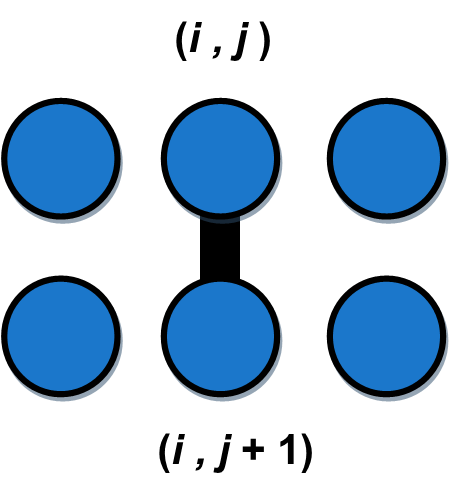
\includegraphics[width=2.5cm]{Figs/Single_couple.png}
   \caption{Single coupling operation.} \label{fig:scheme-single-iteration}
\end{figure}
Note that we do not need to store the exponential operator matrices $\mathrm{e}^{\imath \frac{\alpha}{2} A}$ and $\mathrm{e}^{\imath \frac{\alpha}{2} B}$. It is sufficient to store only two values: $ \cos\left(\frac{\alpha}{2}\right)$ and $\sin\left(\frac{\alpha}{2}\right)$.

Following this scheme, Eq.~\eqref{eq:single-iteration} can be schematized as in Fig.~\ref{fig:scheme-iteration}. The single time evolution is divided in nine computational steps corresponding to the matrix vector multiplications. Furthermore, the operations are independent one another, so that sites in each computational step can be updated in place.
\begin{figure}
   \centering
   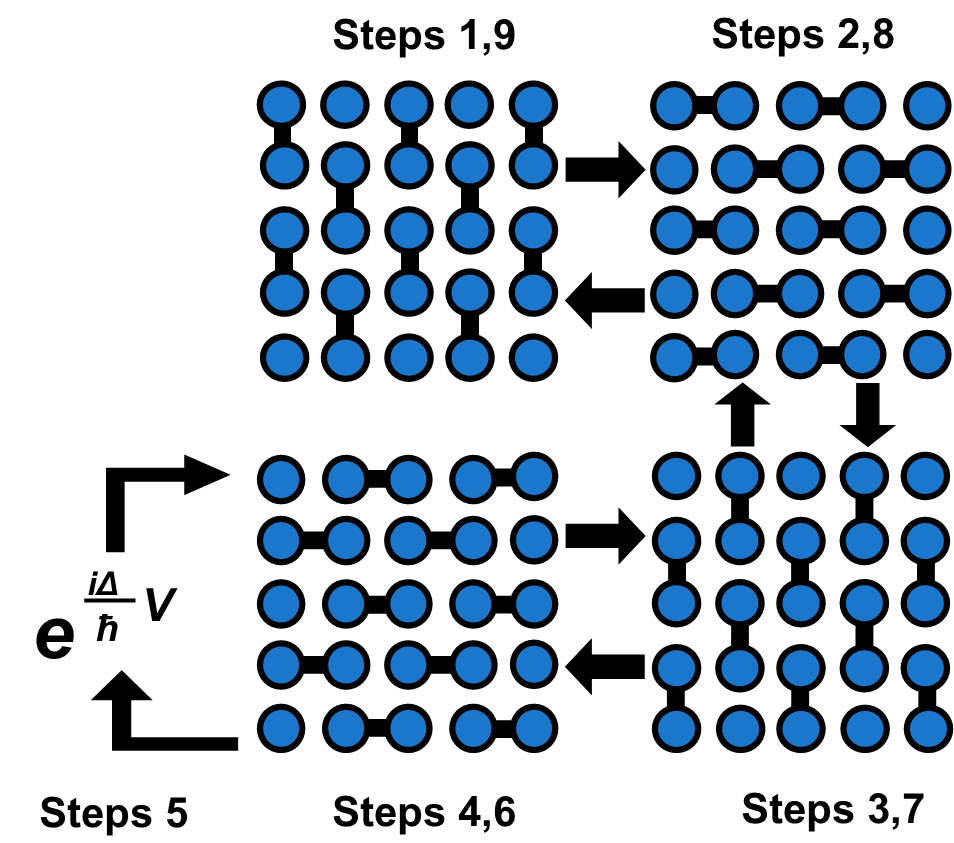
\includegraphics[width=8cm]{Figs/Single_time_step_evolution.png}
   \caption{Single time step evolution scheme for the second order Trotter-Suzuki.} \label{fig:scheme-iteration}
\end{figure}

%%%%%%%%%%%%%%%%%%%%%%%%%%%%%%%%%%%%%%%%%%%%%%%%%%%%%%%%%%%%%%%%%%%%%%%%%%%%%%%%%%%%
\subsection{Cache-aware implementation}
A Naive approach to implement the scheme in Fig.~\ref{fig:scheme-iteration} is by performing each computational step in a single pass over the entire array of sites. This perform efficiently as long as the array of sites fits in the cache, so that the CPU fetch the data directly from the cache. However, for large system sizes, data need to be fetched from the main memory, resulting in a fall of performance~\citep{bederian2011boosting}. 

Cache optimization can be achieved dividing the array of sites in blocks that fit in the cache and performing a single time step evolution for each one of them, separately. This raise the problem of data dependency. Suppose that a block has been read to the cache and evolved a number of steps. We cannot write the results back to the same array in the main memory, from where the block was read, as blocks adjacent to it still need some values on the boundary between the blocks for their own evolution. This is fixed through double buffering, allocating two arrays in the main memory instead of one and going back and forth between the two,reading from one and writing on the other.

Besides, to perform some computational steps on a block, we need the sites surrounding the block to be present in the cache as well, otherwise the sites on the edge of the block will not be valid. This is because each site needs their four neighbours to complete a single time step evolution. As we try to perform more computational steps on a block, the amount of nodes external to the block increases. These nodes generate a \textit{halo} around a block that must also be read into the cache and updated, but that at later steps become invalid because their own halos are not present. The minimum value of the halo thickness for a single time step evolution is of four sites, since there are four computational steps that couple sites for each direction.

In a non distributed version of the kernels a single CPU performs the time step evolutions as schematized in Fig.~\ref{fig:scheme-iteration}. Blocks of the array in the main memory, with their own halo, are written in the cache memory. A single time step evolution of the block is performed, writing the results back to the cache. The halo is discarded, while the block is written to the second buffer in the main memory (Fig.~\ref{fig:CPU-cache-optimization}). The multiple step strategy, combined with the tunable block size that depends on the hardware's cache size, put the algorithm in the family of cache-aware stencil computations~\cite{kamil2006implicit}.
\begin{figure}
   \centering
   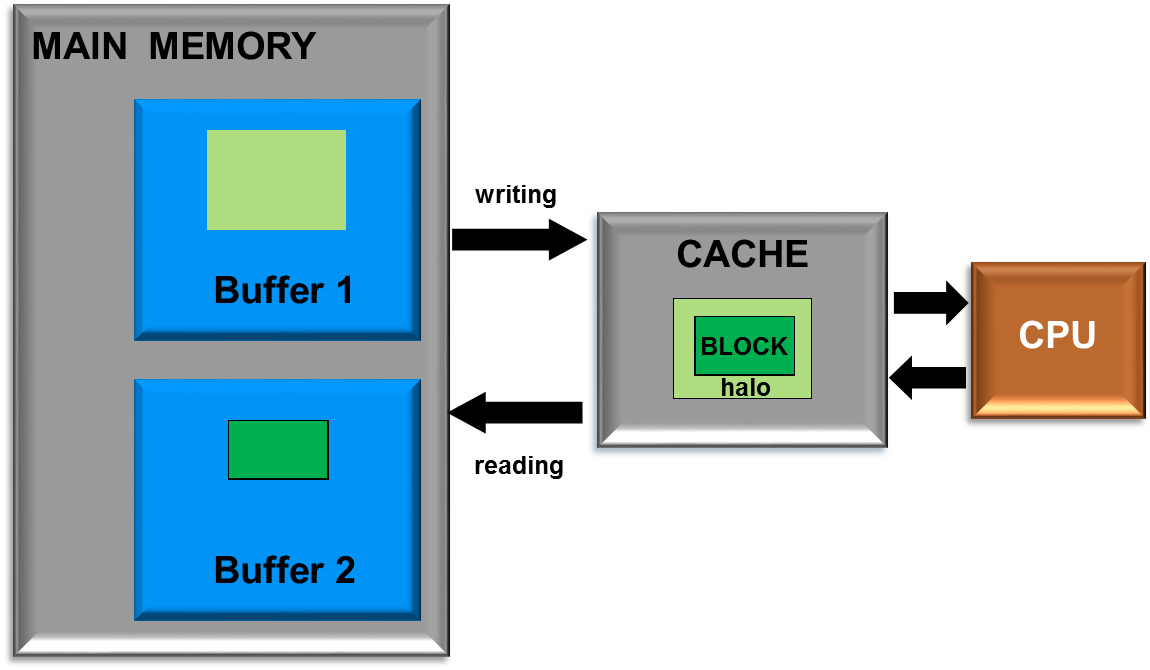
\includegraphics[width=10cm]{Figs/CPU-cache_optimization.png}
   \caption{Scheme of the CPU cache optimization. A time step evolution is performed, writing blocks of the first array into the cache.} \label{fig:CPU-cache-optimization}
\end{figure}

%%%%%%%%%%%%%%%%%%%%%%%%%%%%%%%%%%%%%%%%%%%%%%%%%%%%%%%%%%%%%%%%%%%%%%%%%%%%%%%%%%%%%
\section{GPU kernel}
As the time step evolution is composed by simple and high parallelizable instructions, an implementation that runs on GPU gain a high speed-up compare to a CPU kernel. Indeed, GPUs has gained a much higher computational power with respect to CPU, as illustrated in Fig.~\ref{fig:CPU-GPU-computational-power}. This motivate the development of a GPU kernel. In this section we outline the differences between CPU and GPU, describing the features of the latter. A description of the non distributed version of GPU kernel follows.
\begin{figure}
   \centering
   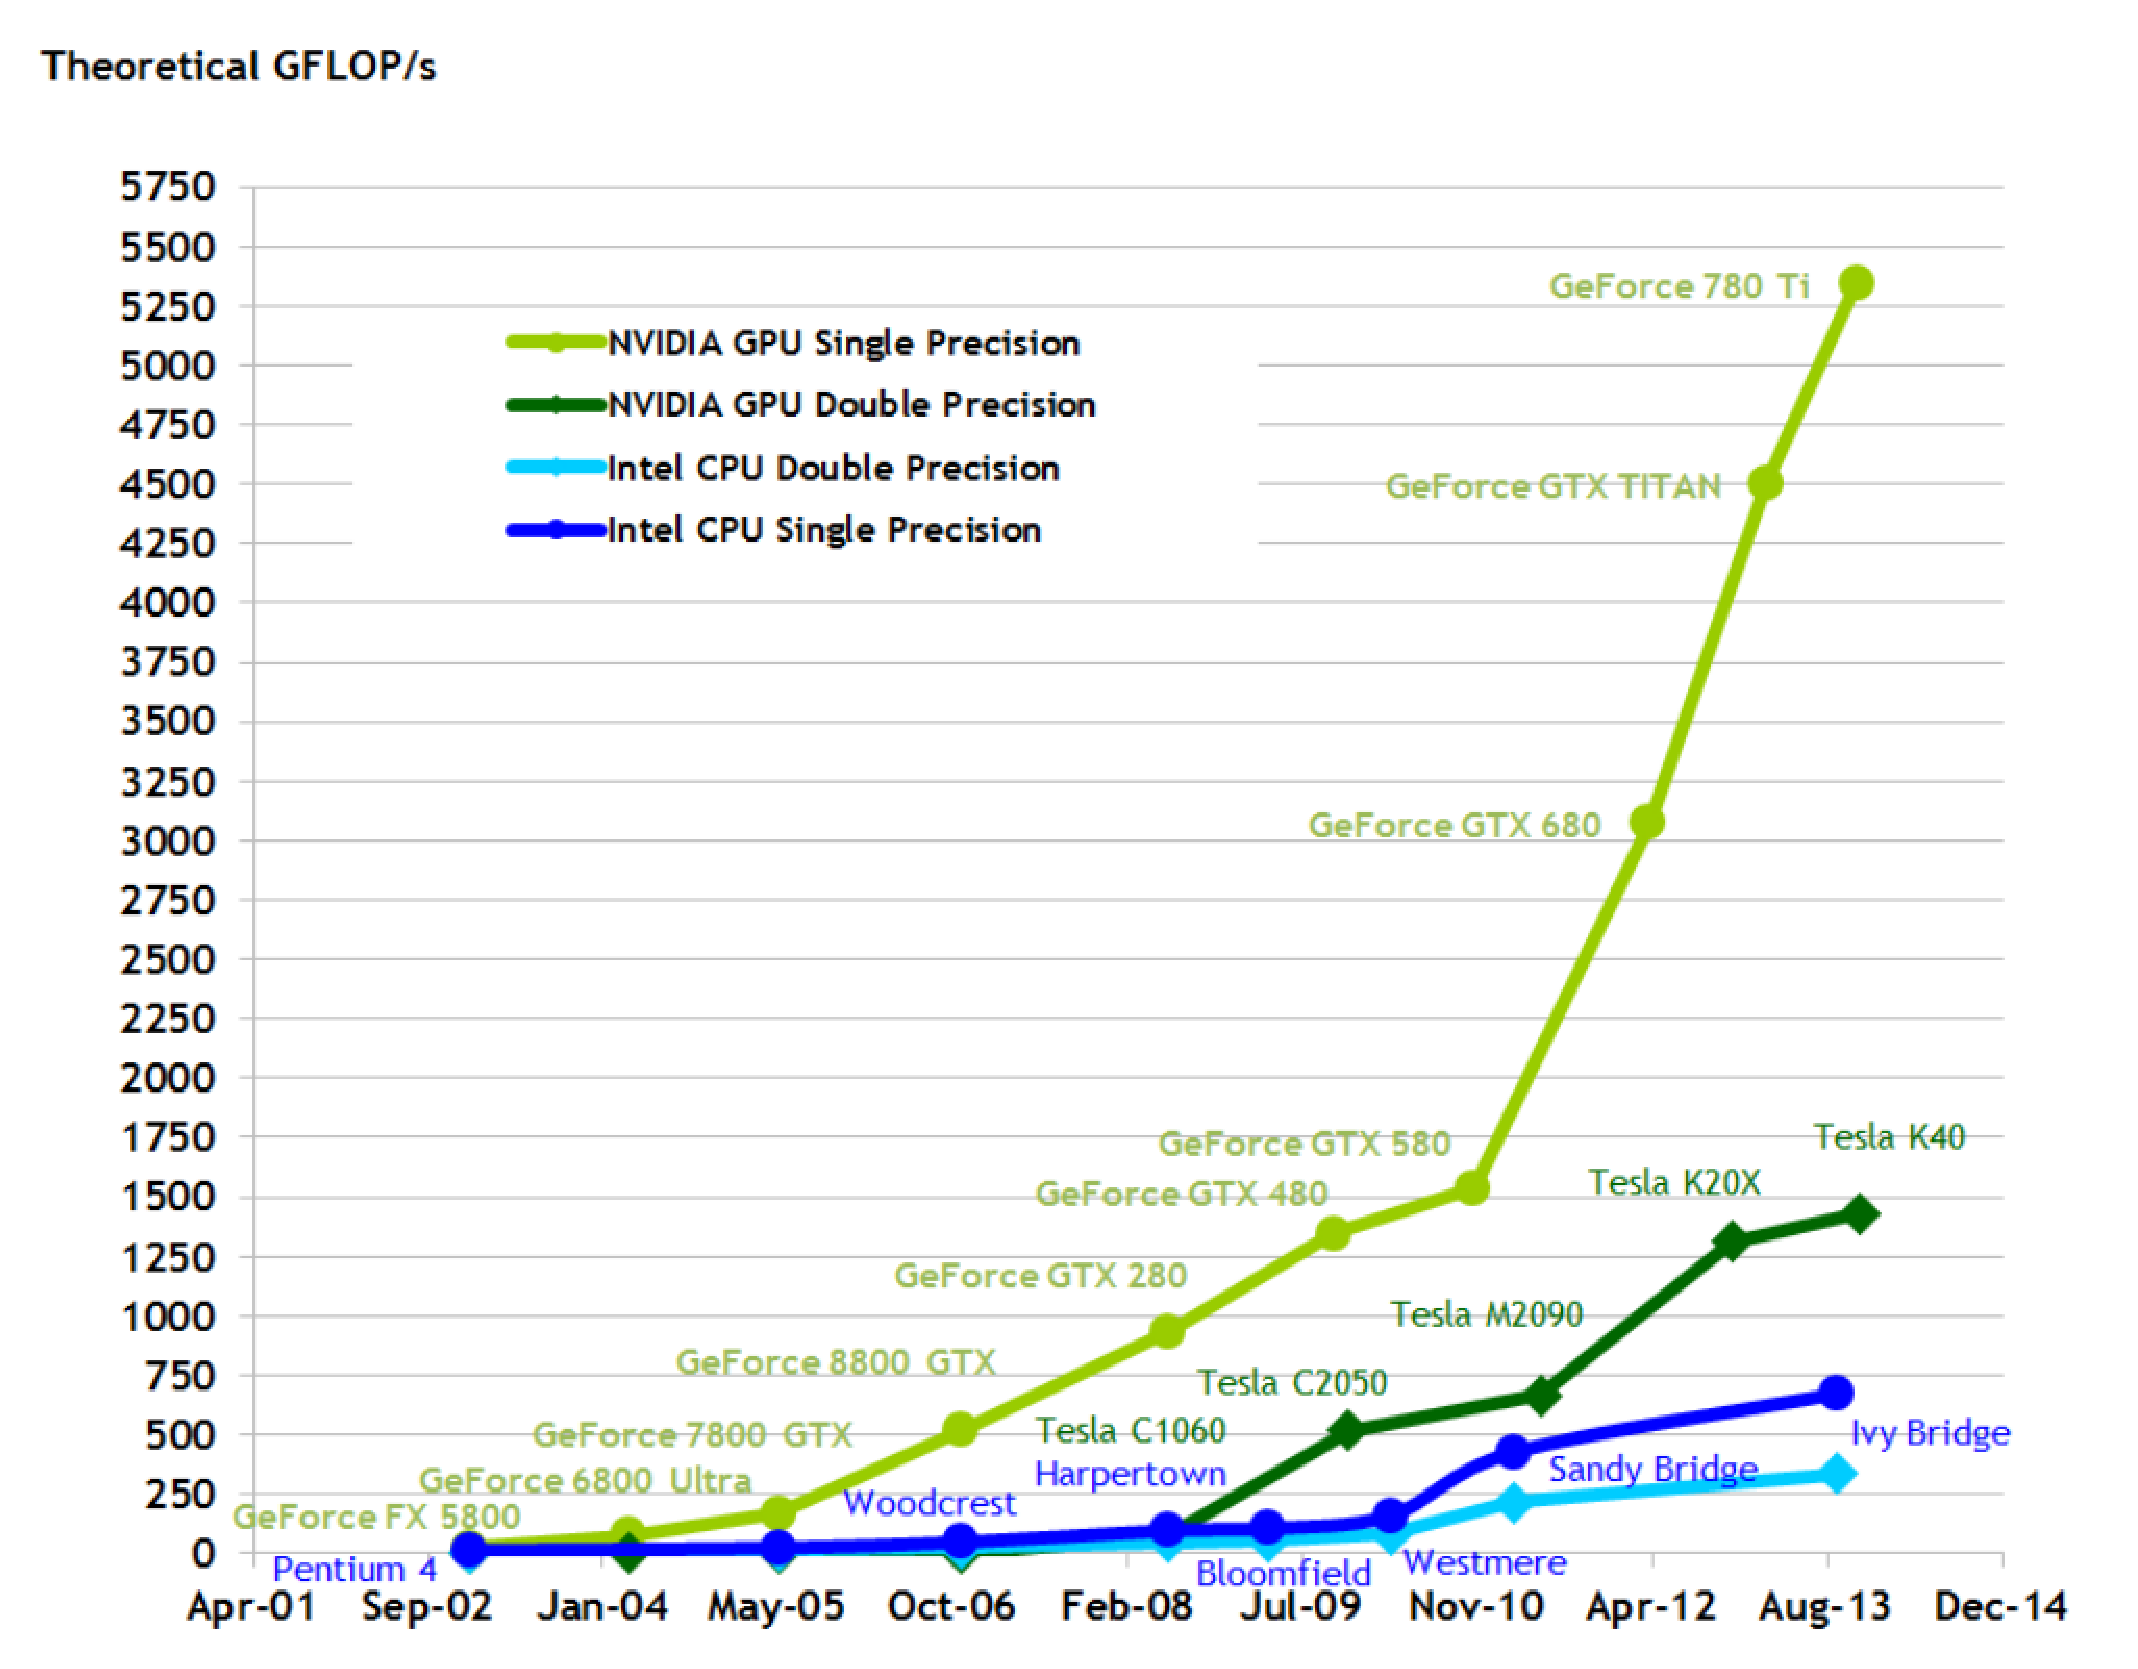
\includegraphics[width=10cm]{Figs/CPU-GPU_computational_power.eps}
   \caption{Floating-point operations per second for the CPU and GPU.} \label{fig:CPU-GPU-computational-power}
\end{figure}

%%%%%%%%%%%%%%%%%%%%%%%%%%%%%%%%%%%%%%%%%%%%%%%%%%%%%%%%%%%%%%%%%%%%%%%%%%%%%%%%%%%%%
\subsection{GPU structure}
The reason behind the discrepancy in floating-point capability between the CPU and the GPU is that the GPU is specialized for compute-intense, highly parallel computation and therefore designed such that more transistors are devoted to data processing rather than data caching and flow control. Indeed, GPU is well-suited to address problems that can be expressed as data-parallel computations, where the same program is executed on many data elements in parallel. Consequently, there is a lower requirement for sophisticated flow control. Furthermore, because the program is executed on many data elements and has high arithmetic intensity, the memory access latency can be hidden with calculations instead of big data caches.

GPUs adopt \textit{SIMT (single instruction, multiple thread)} architecture as parallel execution model. Data elements are processed by sequence of parallel instructions called \textit{threads}. The NVIDIA GPU architecture is built around a scalable array of multithreaded \textit{Streaming Multiprocessors (SMs)}. Threads are managed, created, scheduled and executed by SMs in groups of 32 parallel threads called \textit{warps}. Individual threads composing a warp start together at the same program address, but they have their own instruction address counter and register state and are therefore free to branch and execute independently. When a multiprocessor is given one or more thread blocks to execute, it partitions them into warps and each warp gets scheduled by a warp scheduler for execution. 

A warp executes one common instruction at a time, so full efficiency is realized when all 32 threads of a warp agree on their execution path. If threads of a warp diverge via a data-dependent conditional branch, the warp serially executes each branch path taken, disabling threads that are not on that path, and when all paths complete, the threads converge back to the same execution path (Fig.~\ref{fig:warp-instruction}). Branch divergence occurs only within a warp; different warps execute independently regardless of whether they are executing common or disjoint code paths. Consequently, avoiding threads in a warp to branch, the execution achieve better performance.
\begin{figure}
   \centering
   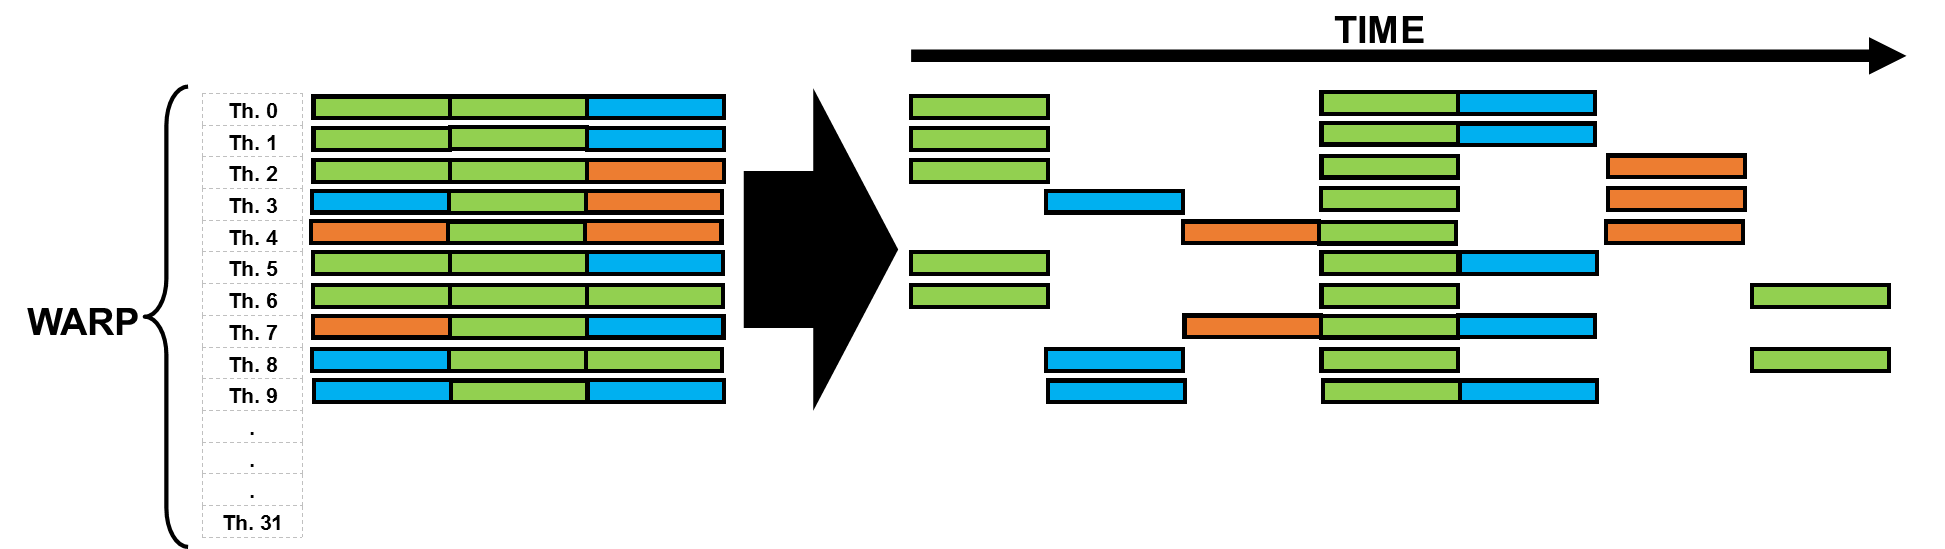
\includegraphics[width=14cm]{Figs/Warp_instruction.png}
   \caption{Instance of a warp execution. The left part of the graph illustrates the instructions to be performed by each thread. Each thread execute three instructions; instructions with the same color are identical. The right part of the graph illustrates how the instructions are executed by the threads within a warp. Threads, that execute the same instruction, perform the instruction at the same time. Different instructions are performed on different times. In this example threads are not in the same execution path -- there are at least three different paths -- resulting in a inefficient time performance.} \label{fig:warp-instruction}
\end{figure}

GPU are easily programmed using \textit{CUDA C} an extension of high-level programming language C. CUDA C extends C by allowing the programmer to define C functions (kernels) that are executed N times in parallel by N different \textit{CUDA threads}. Each thread is associated to a 3-component vector, so that they are organized in a 3d structure. Groups of threads are collected in \textit{thread blocks}, whose size is dictated by the programmer. However, there is a limit to the number of threads per block, since all threads of a block are expected to reside on the same processor core and must share the limited memory resources of that core. Blocks are organized into a \textit{grid} of thread blocks, which can be one, two or three dimensional.

GPU's memory is organized in a hierarchy, as it happens for the CPU (Fig.~\ref{fig:GPU-memory-hierarchy}). Closest to the processors there are fast and small registers, in which each thread store a private local memory space. On the next level in the hierarchy, there are \textit{shared memories}. Each thread block can access to a memory space stored on shared memories, which is visible to all the threads of the block. The last level consist in the global memory, accessible by all the threads.
\begin{figure}
   \centering
   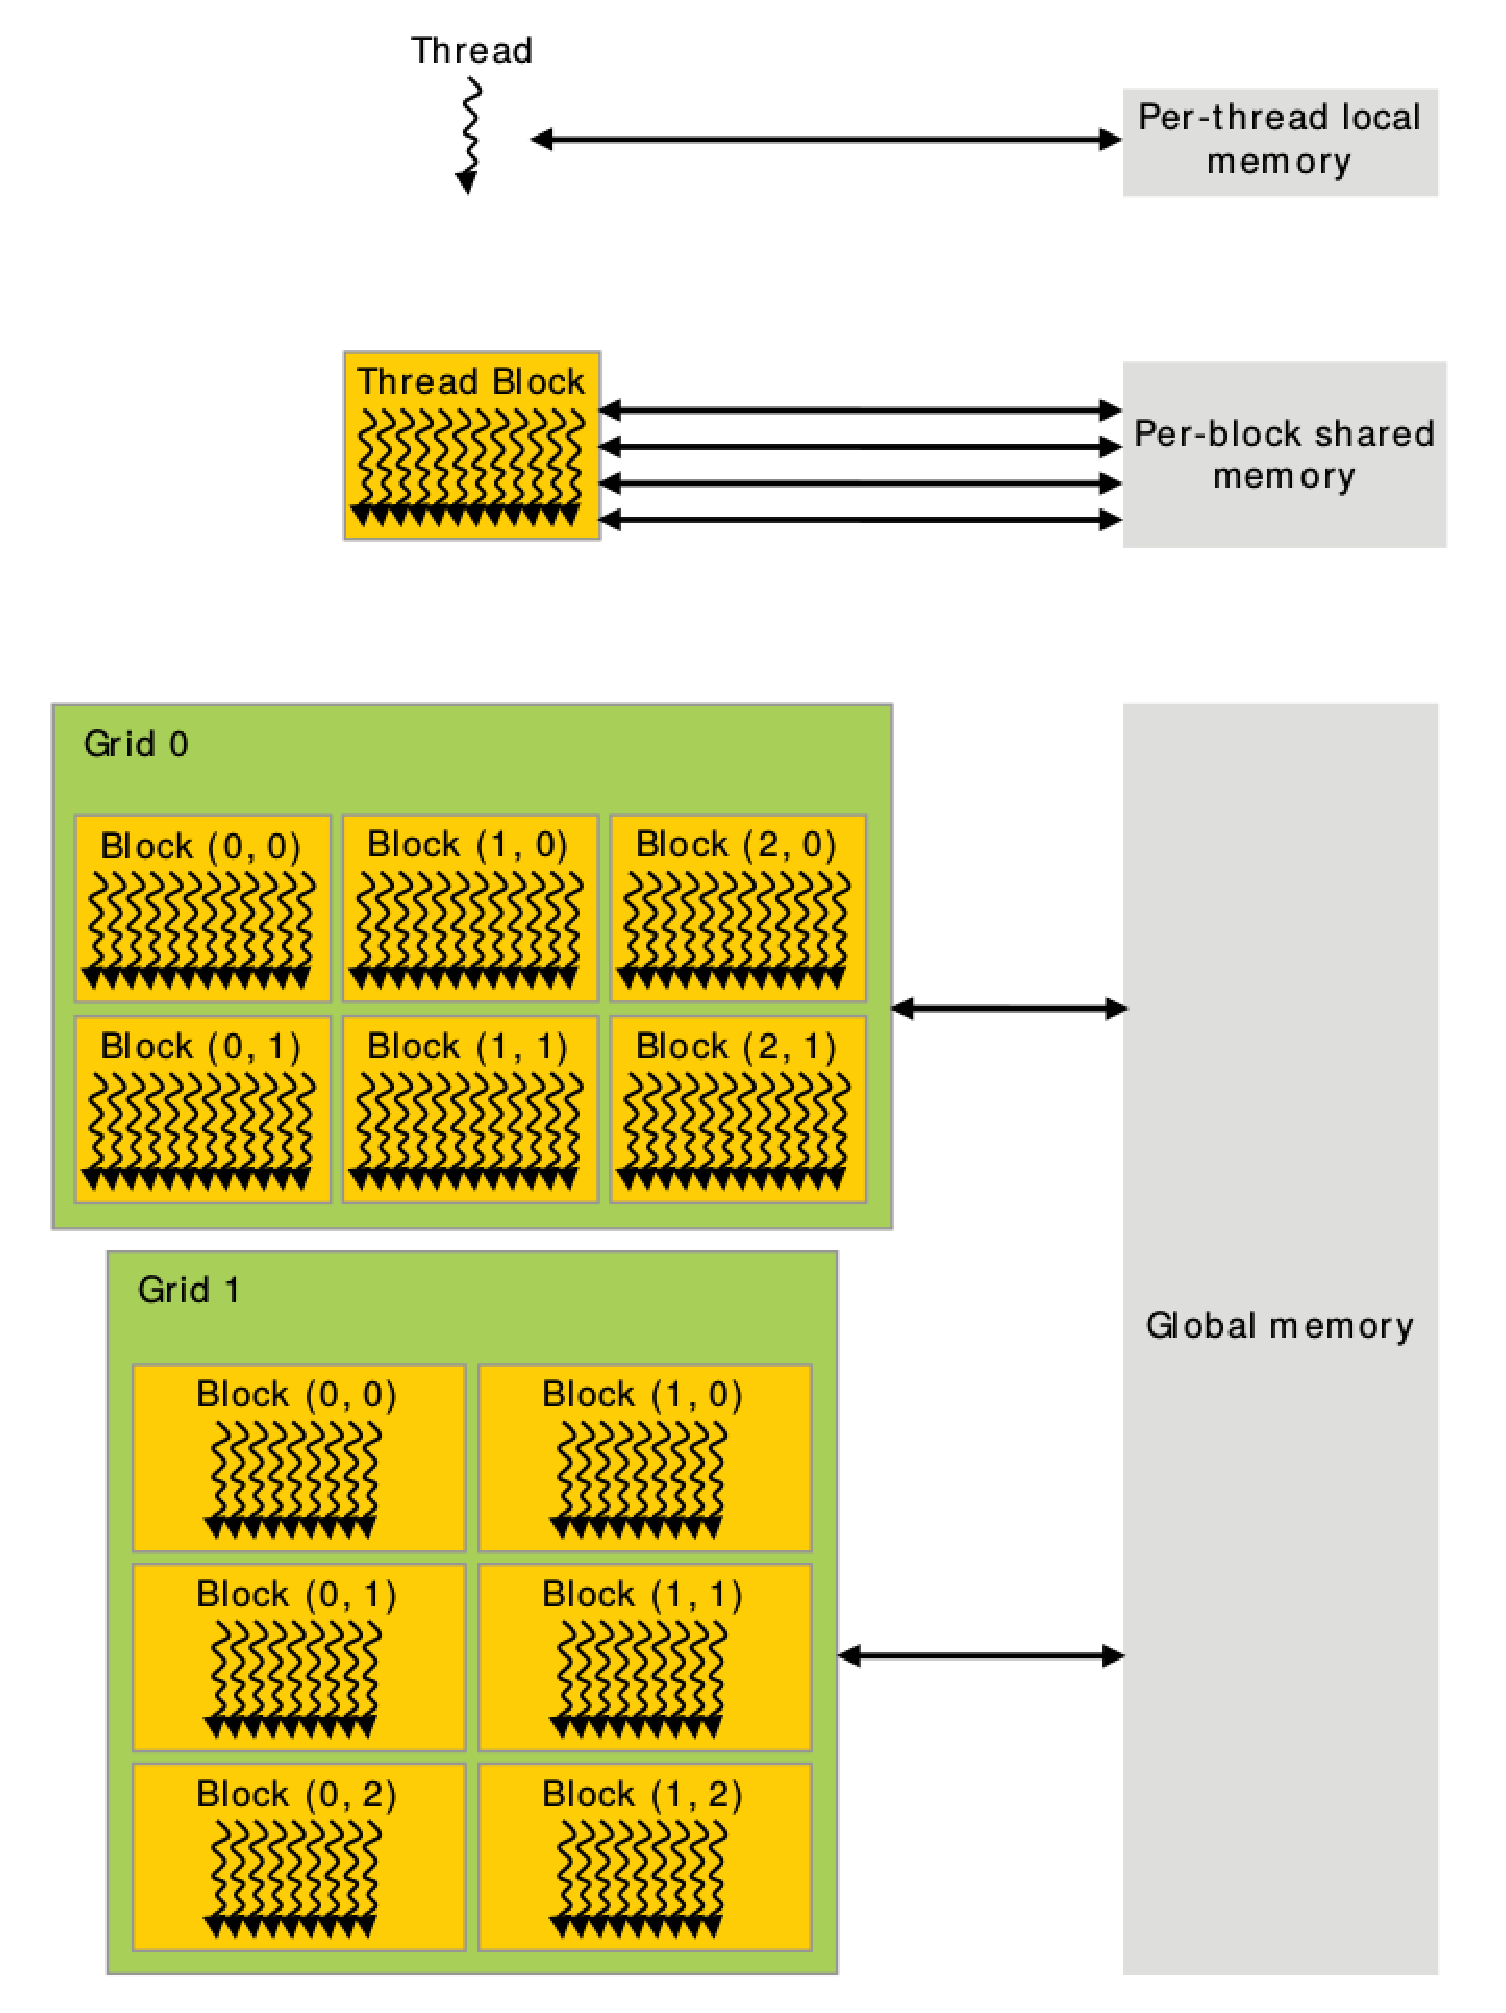
\includegraphics[width=10cm]{Figs/GPU_memory_hierarchy.eps}
   \caption{GPU memory hierarchy.} \label{fig:GPU-memory-hierarchy}
\end{figure}

In the CUDA programming model, the GPU is regarded as a physically separate \textit{device} that operates as a coprocessor to the \textit{host} -- the CPU -- running the C program. This is the case when the kernel executes on a GPU, while the rest of the C program executes on a CPU. The host and the device maintain their own separate memory spaces. Therefore, host and device communicate to share data. In particular, the host can allocate and deallocate space on the device global memory, as well as transfer data between host main memory and device global memory.
%write about heterogeneous programming?

%%%%%%%%%%%%%%%%%%%%%%%%%%%%%%%%%%%%%%%%%%%%%%%%%%%%%%%%%%%%%%%%%%%%%%%%%%%%%%%%%%%%%
\subsection{GPU implementation}
The GPU kernel implements the same time step evolution as the CPU kernel (Fig.~\ref{fig:scheme-iteration}). In analogy with the CPU kernel, the  GPU kernel divides the array of sites in blocks, which are written in the shared memories of the multiprocessors, along with their own halo. This strategy benefits from the higher bandwidth of the shared memories, as it happens for the CPU cache. Double buffering is required for data dependency; two arrays in the global memory are allocated, one for reading and one for writing the results. Besides, blocks are executed in parallel, reducing the time of the execution. 

The time step evolution is performed using half number of threads as there are sites in the shared memory. In particular, each thread executes a single coupling operation. Data are partitioned so that each thread process couples of neighbours sites. This is done by arranging the threads in a checkerboard pattern; each thread allocate in its local memory the element corresponding to its position in the checkerboard, keeping it during all the single time step evolution execution. Then, it updates the value of this element and the one in its neighbour in the shared memory, which is determined by the computational step that is currently executed. The single coupling operations are executed in parallel by the threads, but the computational steps may be processed in a serialized manner, due to data dependency. Thus, after each computational step there is a synchronization barrier. 
%schematic fig

%%%%%%%%%%%%%%%%%%%%%%%%%%%%%%%%%%%%%%%%%%%%%%%%%%%%%%%%%%%%%%%%%%%%%%%%%%%%%%%%%%%%%
\section{Hybrid kernel}
During the execution of the GPU kernel, the host's CPU is idle while waiting for the GPU to complete the calculations. This CPU time could be used to perform part of the evolution of the state. Furthermore, GPU have less memory than CPU, limiting the size of the quantum system for which the evolution is computed. A hybrid kernel that uses both CPU and GPU address these two issues.

The algorithm calculates the maximum amount of the array sites that can be computed on the GPU. Then an internal area of the array site, with the appropriate size, is sent to the GPU to be calculated. Since CPU and GPU are in charge of evolving different area of the array sites, GPU requires an halo surrounding the internal area while the CPU needs the halo that correspond to the sites at the edge of the internal area. A single time step evolution is performed, using the CPU and GPU kernels described above for the corresponding areas. After that, the internal halos must be updated by performing a communication between CPU and GPU. The GPU receives the halo from the corresponding part of the mesh evolved by the CPU -- for the CPU is the other way around. 

The kernel also uses a directive-driven parallelism to utilize the power of a multicore system, relying on OpenMP. In the CUDA programming model, each GPU is associated to a single host, which is a single CPU core, hence, in a system with multicore CPU and a single GPU, only one single CPU would be used. For this purpose, the CPU kernel is slightly adjust to use OpenMP, so that the blocks which divides the CPU mesh are processed in parallel using more than one CPU.

%%%%%%%%%%%%%%%%%%%%%%%%%%%%%%%%%%%%%%%%%%%%%%%%%%%%%%%%%%%%%%%%%%%%%%%%%%%%%%%%%%%%%
\section{Distributing the workload across a cluster}
The code is designed to run also in a distributed multi-node system. The whole mesh is partitioned in blocks, called tiles. Each node processes a tile plus its halo. After a single time step evolution the halos between the tiles have to be sent across the nodes. The communication is implemented using MPI. Using a two-dimensional grid of nodes, a tile contains elements of halos belonging to a total of eight other tiles: left, right, top, and bottom neighbours, and also the four diagonal neighbours. To minimize the number of communication requests, a wave pattern is used in the communication: left and right neighbours receive the halo first. This halo has the height of the inner cells of the tile. Then the horizontal halos are sent to the top and bottom neighbours – the width is the full tile width. In this way the appropriate corner elements are propagated to the diagonal neighbours.

The communication is performed asynchronously: each halo is sent at the same time. However, there is a communication barrier between the left-right and top-bottom halo exchange due to data dependency. To achieve better performance, the approach is to overlap communication and evolution as much as possible, evolving the halo first and starting the communication simultaneously to the evolution of the rest of the tile. 

The CPU kernels evolve blocks of the tile at its edge, corresponding to the halos. Then the asynchronous left-right halo exchange and the evolution of the inner part of the tile initiates. Once finished the evolution of the inner part, there is the left-right halo exchange barrier. Consequently, the asynchronous top-bottom halo exchange starts and the top-bottom barrier ensure that it finish before swapping the buffers and continuing with the next time step. In this case, the halo exchange cannot be efficiently overlapped with computation, since, after the time step evolution is finished, there is a communication overhead while the vertical halos are exchanged.

As regard the GPU kernel, the communication is performed from the host memory. This increases the complexity, as asynchronous memory copies from the device and to the device have to be performed. To work with such transfer efficiently, the kernel implements \textit{streams}. A GPU stream is basically a queue of tasks for the GPU to perform: kernel execution, and memory copies from and to the device. Tasks in two different streams can overlap with each other, while tasks on the same stream are performed sequentially. When the host queues a task into a GPU stream, it does not have to wait for the task to be completed by the GPU before continuing with the rest of the algorithm. Two streams are implemented in the kernel: queueing the halo computation and the memory copies between host and device in stream one, and the computation of the inner part of the tile in stream two.

The host start queueing the evolution of the blocks at the edge of the tile, corresponding with the halo, and the halo copy from device to host in stream one. While the GPU is running the first stream, the host queues the evolution of the rest of the blocks in the second stream. Once the GPU finish the tasks in the first stream the halo can be exchanged between the nodes, using the wave pattern described above. With this approach, the communication of all halos is efficiently overlapped with the blocks calculation -- the task in the second stream. When the halo communication is completed, the host queues the copy of the halos received to the device memory in the first stream. Once the GPU finishes the tasks in each streams, the buffers in the global memories are swapped and the kernel starts over.

We say that certain GPUs allow device-to-device transfer without involving the host memory, and some configurations also allow similar transfers between GPUs located in different hosts. We assumed that GPU-GPU communication would always involve the host memory.

We use one process per GPU, and single-node execution with multiple GPUs is possible.

The hybrid kernel uses only one stream to queue the tasks for the GPU. The host launch the GPU kernel for the corresponding sites on the internal area of the tile. After that the host -- CPU -- proceeds to calculate the halo and start the halo exchange. Once the halo exchange is initiated, the sites not in the halo and not on the GPU are evolved by the CPU. Finally, finished the halo exchange, it exchange the internal halo between the part of the tile associated with the GPU and the rest of the matrix.

\chapter{Dark Solitons in Bose--Einstein Condensates}
\chaptermark{Dark Solitons in BEC}
As a case study of the code developed, we carried out simulations of the dynamics of a Bose--Einstein condensate (BEC). In particular we reproduced the results of an experimental study performed at the National Institute of Standards and Technology (NIST), in which they investigated the realization and evolution of solitons in a BEC of sodium atoms~\citep{DSF00}. In this chapter we briefly introduce the theoretical background of BEC and dark solitons, and proceed with the illustration of the simulation results, comparing them to the results by NIST.

%%%%%%%%%%%%%%%%%%%%%%%%%%%%%%%%%%%%%%%%%%%%%%%%%%%%%%%%%%%%%%%%%%%%%%%%%%%%%%%%%%%%
\section{Theoretical Background}
The dynamics of a weakly interacting Bose--Einstein condensate may be described by a nonlinear Schr\"odinger equation, namely, the Gross--Pitaevskii equation~\citep{pethick2002bose,DGPS99,LSA12}. Suppose we have a N--particle system, comprised of bosons interacting with each other. Using the Hartree approximation, we write the many--body wave function as
\begin{equation}
\psi(\textbf{r}_1, \textbf{r}_2,\ldots, \textbf{r}_N) = \prod_{i=1}^N \phi(\textbf{r}_i),
\end{equation}
where the single--particle wave function $\phi(\textbf{r}_i)$ is normalized in the usual way,
\begin{equation}
\int \mathrm{d}\textbf{r} \, |\phi(\textbf{r})|^2 = 1.
\end{equation} 
For low energy particles, the interaction can be described by an effective potential
that in coordinate space corresponds to a contact interaction $U_0 \delta(\textbf{r} - \textbf{r}')$, where $U_0 = 4 \pi \hbar^2 a_s / m$ and $a_s$ is the scattering length of the interaction~\citep{pethick2002bose}. Considering an external potential $V(\textbf{r}_i)$, the Hamiltonian may be written as
\begin{equation}
H = \sum_{i=1}^N \left[ \frac{\textbf{p}_i^2}{2 m} + V(\textbf{r}_i) \right] + U_0 \sum_{i<j} \delta(\textbf{r}_i - \textbf{r}_j).
\end{equation}
Then, the energy of the state is given by
\begin{equation}
E =  N \int \mathrm{d} \textbf{r} \, \left[ \frac{\hbar^2}{2m} |\nabla \phi(\textbf{r}) |^2 + V(\textbf{r}) |\phi(\textbf{r})|^2 + \frac{(N-1)}{2} U_0 |\phi(\textbf{r})|^4 \right].
\end{equation} 
It is convenient to introduce the concept of the wave function of the condensed state,
\begin{equation}
\psi(\textbf{r}) = N^{1/2} \phi(\textbf{r}),
\end{equation}
so that the normalization condition becomes
\begin{equation} \label{eq:normalization-N}
\int \mathrm{d}\textbf{r} \, |\psi(\textbf{r})|^2 = N.
\end{equation}
Moreover, we suppose that $N \gg 1$ so that the energy can be rewritten as,
\begin{equation}
E = \int \mathrm{d} \textbf{r} \, \varepsilon  = \int \mathrm{d} \textbf{r} \, \left[ \frac{\hbar^2}{2m} |\nabla \psi(\textbf{r}) |^2 + V(\textbf{r}) |\psi(\textbf{r})|^2 + \frac{1}{2} U_0 |\psi(\textbf{r})|^4 \right].
\end{equation}
The equation of motion may be derived from the principle of least action 
\begin{equation}
\delta \int_{t1}^{t2} \mathrm{d} t \, L = 0 \label{eq:least-principle}
\end{equation}
where the Lagrangian $L$ is given by
\begin{equation}
L = \int \mathrm{d} \textbf{r} \, \left[ \frac{\imath \hbar}{2} \left( \psi^\ast \frac{\partial \psi}{\partial t} - \psi \frac{\partial \psi^\ast}{\partial t} \right) - \varepsilon \right].
\end{equation}
Requiring that the variation of the independent variables $\psi(\textbf{r},t)$ and $\psi^\ast (\textbf{r},t)$ vanishes at $t=t_1$ and $t=t_2$, and on any spatial boundaries, from Eq.~\eqref{eq:least-principle} one finds the Gross--Pitaevskii equation:
\begin{equation} \label{eq:gross-pitaevskii}
\imath \hbar \frac{\partial \psi(\textbf{r}, t)}{\partial t} = \left[ - \frac{\hbar^2}{2m} \nabla^2 + V(\textbf{r}) + U_0 |\psi(\textbf{r}, t)|^2 \right] \psi(\textbf{r}, t).
\end{equation}

Formally, Eq.~\eqref{eq:gross-pitaevskii} is not implemented in our code since the Hamiltonian is not simply comprised of a kinetic term and an external potential term. However, if we denote $\tilde{V}(\textbf{r}, \psi(\textbf{r}, t)) = V(\textbf{r}) + U_0 |\psi(\textbf{r}, t)|^2$, the single time step evolution still has the form~\eqref{eq:single-iteration} and the exponential operator $\exp \left( - \frac{\imath}{\hbar} \tilde{V}(\textbf{r}, \psi(\textbf{r}, t)) \right)$ is still diagonal in the coordinate representation. Thus, we only have to define the potential such that, in the computational step 5 (Fig.~\ref{fig:scheme-iteration}), each site $(i,j)$ is also multiplied by the factor $\exp(-\frac{\imath}{\hbar} U_0 |\psi(i,j)|^2)$ where $\psi(i,j)$ is the wave function calculated in the previous computational step.

The ground--state of the system may be found numerically using the imaginary time evolution. However, for sufficiently large number of atoms an accurate expression is obtained using the Thomas--Fermi approximation. Suppose that the contribution of the kinetic energy term is negligible with respect to the one of the interaction terms. Then the ground--state is approximated by the solution of the time independent Gross--Pitaevskii equation deprived of the kinetic term
\begin{equation}
\left[ V(\textbf{r}) + U_0 |\psi(\textbf{r})|^2 \right] \psi(\textbf{r}) = \mu_{TF} \psi(\textbf{r}),
\end{equation}
where $\mu_{TF}$ is the chemical potential. This gives the solution
\begin{equation}
n(\textbf{r}) = |\psi(\textbf{r})|^2 = \frac{\mu_{TF} - V(\textbf{r})}{U_0},
\end{equation}
%check if I need to put abs in U_0
for $\textbf{r}$ such that $V(\textbf{r}) < \mu_{TF}$. 
For a BEC trapped in a harmonic potential of the form
\begin{equation}
V(x,y) = \frac{m}{2} (\omega_1^2 x^2 + \omega_2^2 y^2)
\end{equation}
the extension of the condensate wave function in the two directions is given by the two semi--axes
\begin{equation} \label{eq:TF-radius}
R_i = \sqrt{\frac{2\mu_{TF}}{m\omega_i^2}}, \quad i = 1,2 ,
\end{equation}
and the particles density has the form of an inverted parabola. Given the normalization condition in Eq.~\eqref{eq:normalization-N}, the chemical potential is determined as a function of $U_0$ and the system dimension (see Appendix~\ref{App:A}).

The Thomas--Fermi approximation gives an accurate description of the bulk properties of the system, but it fails near the edge of the cloud. Provided that $V(\textbf{r})$ varies slowly, a better solution for the ground state may be found solving the entire time independent Gross--Pitaevskii equation taking the linear term of the external potential at the edge of the cloud~\citep{pethick2002bose}.

The Gross--Pitaevskii equation has exact analytical solutions in the nonlinear regime. These solutions have the form of solitary waves, called solitons, which are localized disturbances that propagate without changing of form~\citep{RC97,JKP98,DCLZ98,ZPMW99}. This phenomenon is due to the balance between dispersion and nonlinearity, which in Eq.~\eqref{eq:gross-pitaevskii} correspond to the kinetic term and the nonlinear interaction, respectively. Solitons appear in different contexts of science and engineering, such as the dynamics of waves in shallow water~\citep{B88}, transport along DNA and other macromolecules~\citep{P95}, and fiber optic communications~\citep{H90}.
Depending on the details of the governing nonlinear equation, they can be either bright or dark. The former are peaks in the amplitude, while the latter are notches with a characteristic phase step across. In the present work we focus on dark solitons. 

For BEC with repulsive interaction between the atoms, solitons present a depression in the density profile -- a dark soliton. In a homogeneous BEC, the resulting density profile along the $x$ axis is
\begin{equation}
n(x,t) = n_{min} + \left(n_0 - n_{min}\right)\tanh^2 \left( \frac{x - \nu_s t}{\sqrt{2} \xi} \sqrt{1 - \left( \frac{\nu_s}{\nu_0} \right)^2 } \right)
\end{equation}
where $n_0$ is the unperturbed density, $n_{min}$ is the density at the center of the soliton, $\nu_s$ and  $\nu_0 = (\frac{nU_0}{m})^{\frac{1}{2}}$ are the speed of the soliton and the speed of sound respectively, and 
\begin{equation}
\xi = \frac{\hbar}{\left( 2mn_0 U_0 \right)^{1/2}}
\end{equation}
being the healing length~\citep{pethick2002bose}. The speed and the depth of the soliton can be related with each other~\citep{RC97,JKP98}. Indeed, the soliton speed $\nu_s$ can be expressed as
\begin{equation} \label{eq:soliton-speed-density}
\nu_s = \nu_0 \sqrt{ \frac{n_{min}}{n} }.
\end{equation}
Note that the soliton speed is less than the speed of sound; feature that distinguish it from sound waves and excitations. The soliton speed can also be expressed by means of the change in phase of the wave function across it:
\begin{equation}
\nu_s = \nu_0 \cos \left( \frac{\delta}{2} \right).
\end{equation}

Remarkably, the motion of a soliton in a BEC in an external potential is the same as that of a particle of mass $2m$ in the same potential~\citep{pethick2002bose}. Consequently, for a potential having a minimum, the period of the motion of a soliton is $\sqrt{2}$ times that of a particle of mass $m$ in the potential.

%%%%%%%%%%%%%%%%%%%%%%%%%%%%%%%%%%%%%%%%%%%%%%%%%%%%%%%%%%%%%%%%%%%%%%%%%%%%%%%%%%%%%
\section{Soliton Simulation}
In the experiments carried out in Ref.~\citep{DSF00}, the generation and propagation of solitons were studied in BEC of sodium atoms, confined in a magnetic trap. The magnetic trap generated a harmonic external potential with frequencies $\omega_x = \sqrt{2}\omega_y = 2 \omega_z = 2 \pi \cdot 28$~Hz, while the system were composed by  $1.7 (\pm 0.3) \cdot 10^6$ atoms in the $3S_{1/2}$, $F=1$, $m_F=-1$ state. In this configuration the scattering length is $2.75$~nm~\citep{DSF00}. 

In this experiment, the system is three--dimensional, while our implementation is designed for a two--dimensional system. This would not be a problem if the dynamics of the 3D system was described by three decoupled equations, so that we could independently solve the two corresponding to the variables that span a 2D plane and ignore the other one. The Gross--Pitaevskii equation \eqref{eq:gross-pitaevskii} cannot be decoupled due to the non linear term, so this does not apply to our case. However, our purpose is to study the evolution of a soliton which propagates in one dimension, so we can ignore the dynamic along one of the two dimensions perpendicular to the axis of propagation. An approach to reduce to a two dimensional problem is to make a phenomenological hypothesis about the form of the solution. In the literature~\citep{JKP98,SZ98,Sal01,SPR02,MM03}, one can find several methods to reduce a 3D problem to a 2D one; we adopt the method described in~\citep{PietroMassignan}. The condition is that the solution of the reduced system has the same spatial extent of the original one. Since the 3D system is well described by the Thomas--Fermi approximation\footnote{The experimental configuration satisfies the conditions to adopt the Thomas--Fermi approximation, namely the BEC is close to the ground state with a large number of atoms, so that kinetic energy term is by far lower than the interaction energy term}, the extension of the ground state is known (Eq.~\eqref{eq:TF-radius}). Then, the approach is to rewrite the coupling constant $U_0^{(2)}$ for the 2D system, such that the chemical potential for the 2D system is the same as the one of the 3D system. This will ensure that the spatial extension of the 2D system will be the same as the 3D system (see Appendix~\ref{App:A}). For our simulation we reduced the dimension keeping the $x$ and $y$ axes of the 3D system. The resulting Gross--Pitaevskii equation for the 2D system becomes:
\begin{equation} \label{eq:gross-pitaevskii-simulation}
\imath \hbar \frac{\partial \psi(\textbf{r}, t)}{\partial t} = \left[ \sum_{i=1}^2 \left( -\frac{\hbar^2}{2m} \frac{\partial^2}{\partial x_i^2} + \frac{m}{2} \omega_i^2 x_i^2 \right) + U_0^{(2)} |\psi(\textbf{r}, t)|^2 \right] \psi(\textbf{r}, t),
\end{equation}
where
\begin{equation}
U_0^{(2)} = \frac{\pi}{2} \frac{\mu_{TF}}{N} \left( \bar{R}_{TF} \right)^2 ,
\end{equation}
with $\bar{R}_{TF} = \sqrt{2\mu_{TF} / m \bar{\omega}^2}$ being the mean Thomas--Fermi radius, $\bar{\omega} = \sqrt{ \omega_x \omega_y}$ the geometric mean of the frequencies,
and $\mu_{TF}$ is the chemical potential in the Thomas--Fermi approximation for the 3D system given by
\begin{equation}
\mu_{TF} = \frac{1}{2} \left( 15 N \hbar^2 \omega_x \omega_y \omega_z \sqrt{m} a_s \right)^{2/5}
\end{equation}
\\

\noindent \textbf{Ground state.} According to the experiment, the BEC is initially described by the ground state  of Eq.~\eqref{eq:gross-pitaevskii}. They found it to have a spatial extension described by the Thomas--Fermi diameters of $2R_{TF, x} = 45$~$\mathrm{\mu m}$, $2R_{TF, y} = 64 $~$ \mathrm{\mu m}$ and $2R_{TF, z} = 90 $~$ \mathrm{\mu m}$, with a uniform phase~\citep{DGPS99}.
In the simulation, we approximated the ground state of Eq.~\eqref{eq:gross-pitaevskii-simulation} using imaginary time evolution. We proceeded by taking a Gaussian initial state, evolving it in imaginary time for a fixed number of iterations and then calculating the energy of the resulting state. Repeating this procedure using as initial state the one resulting from the last iteration, the energy decreases converging to the ground state energy. If we call $E_i$ the energy of the state resulting from the iteration $i$, we stopped the procedure once the $i-$th state satisfied the convergence condition
\begin{equation}
\left| \frac{E_{i} - E_{i-1}}{E_{i-1}} \right| < 10^{-6}.
\end{equation}
This ensure that the $i-$th state is an accurate approximation of the ground state. In Fig.~\ref{plot:density_x} and Fig.~\ref{plot:density_y} the profiles of the particle density along the two axes are shown. The particles density of the calculated ground state is in good agreement with the particles density of the Thomas--Fermi approximation and with the experimental results.
%try to put the images side-by-side
\begin{figure}[t!]
   \centering
   \begin{tabular}{c}
      \subfloat[]{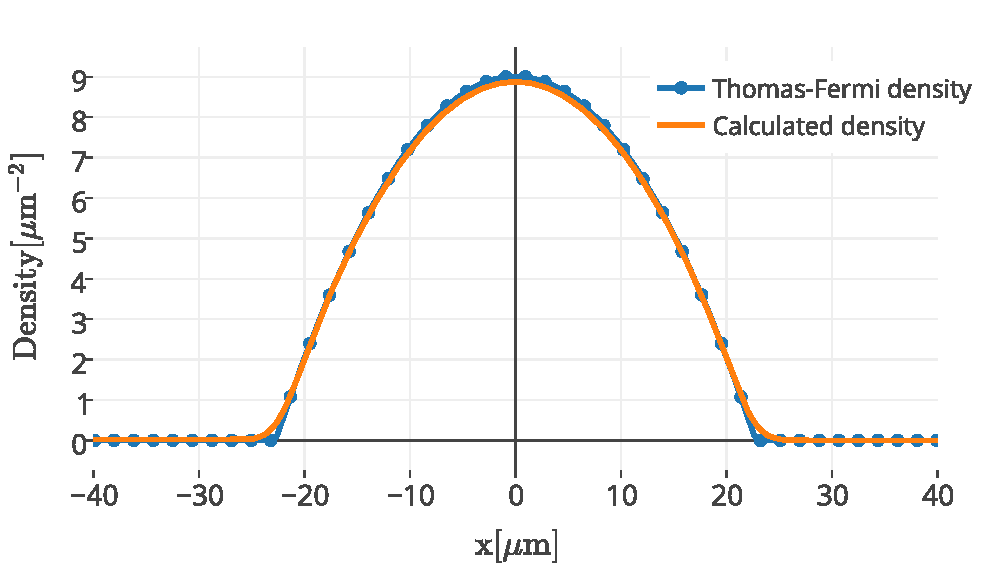
\includegraphics[width=8.5cm]{Plots/density_profile_x.pdf} \label{plot:density_x}} \\
      \subfloat[]{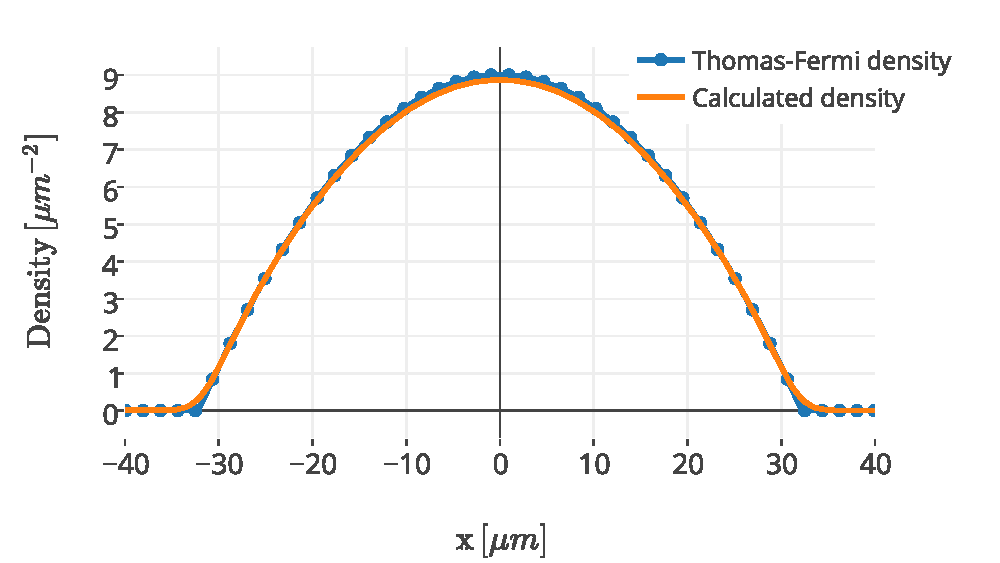
\includegraphics[width=8.5cm]{Plots/density_profile_y.pdf} \label{plot:density_y}} \\
   \end{tabular}
   \caption{Calculated ground--state density along the $x$ axis (a) and the $y$ axis (b). The simulation is in good agreement with the Thomas--Fermi approximation. The spatial extension of the  calculated ground state corresponds to the experimental results, where $R_{TF,x} =  45 $~$ \mathrm{\mu m}$ and $2R_{TF, y} = 64$~$ \mathrm{\mu m}$.}
\end{figure}
\\

\noindent \textbf{Soliton propagation.} Solitons can be generated in BEC by phase imprinting. The phase of the ground state is modified by exposing the cloud to pulsed, off--resonant laser light with an intensity pattern $I(x,y)$. The wave function acquires a corresponding phase $\phi(x,y)$ proportional to $I(x,y)$ and the time of exposure $T$. According to the experiment, they chose $T$ to be short enough so that the atomic motion was negligible (Raman--Nath regime). In this condition, the effect of the pulse can be expressed as a sudden phase imprint, $\psi \rightarrow \psi \exp(\imath \phi(x,y))$~\citep{DSF00}. If the center of the BEC correspond to the origin of the axes, the phase imprint performed in~\citep{DSF00} can be approximated as
\begin{equation}
\phi(x,y) = \frac{\phi_0}{2} \left[1 + \tanh\left(\frac{x}{l}\right)\right],
\end{equation}
where $\phi_0 = 1.5\pi$ and $l=2 $~$ \mathrm{\mu m}$. 

According to the experimental configuration, we set our simulation taking as initial state the transformed ground state $\tilde{\psi}_{gs}$, namely
\begin{equation}
\tilde{\psi}_{gs} = \psi_{gs} \exp(\imath \phi(x,y))
\end{equation}
where $\psi_{gs}$ is the ground state calculated with imaginary time evolution.

The phase imprinting correspond to impressing a momentum to a static ground state, in the region of space where the phase varies. This leads to a collective motion of the system, which corresponds to an oscillation of the BEC along the $x$ axis. This can be seen in the simulation. Fig.~\ref{plot:oscillation} illustrates how the expectation value of the position along the $x$ axis varies in time. As expected from the theory, the oscillation along the $x$ axis has the same frequency as the harmonic potential $\omega_x$, while the position along the $y$ axis remains stable. We found a frequency of $\omega_x = 2 \pi \cdot 27.9$~Hz, in agreement with the experimental value.
\begin{figure}[t]
    \centering
	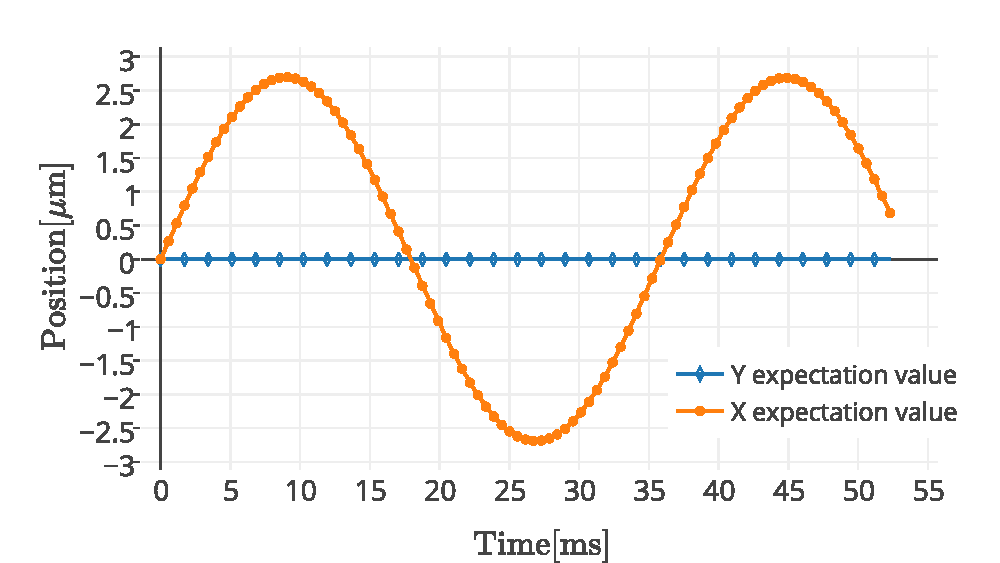
\includegraphics[width=10cm]{Plots/oscillation.pdf}
	\caption{Calculated expectation values $\braket{X}(t)$ and $\braket{Y}(t)$. The calculated oscillation frequency along the $x$ axis, $\omega_x = 2 \pi \cdot 27.9 $~$ \mathrm{Hz}$, is in agrement with the external potential frequency $\omega_x = 2 \pi \cdot 28 $~$ \mathrm{Hz}$. There is no oscillation along the $y$ axis since no impulse is imparted in this direction.} \label{plot:oscillation}
\end{figure}

To observe soliton propagation they exploited absorption imaging, measuring the BEC density distribution. Immediately after the phase imprint, they observed a positive  density disturbance travelling in the $+x$ direction, and a dark notch left behind it, which travels in the opposite direction -- this is the soliton (Fig.~\ref{plot:density_exp_1ms} to~\ref{plot:density_exp_10ms}). The positive disturbance travels with a speed higher than the soliton.

They determined the soliton speed along the $x$ axis, measuring the distance after $5 $~$ \mathrm{ms}$ of propagation between the notch and the position of the imprinted phase step. At that time the soliton had not travelled far from the BEC center, so this is a good estimation of the soliton speed at the center of the condensate. They obtained a mean soliton speed of  $1.8 \pm 0.4$~mm/s. This value is lower than the mean speed of sound $\nu_0 = 2.8 \pm 0.1$~mm/s, which ensures that the dark notch is a soliton and not a sound wave~\citep{DSF00}. In our simulation, we tracked the position of the soliton along the $x$ axis for $14$~ms (Fig.~\ref{plot:soliton-xposition}). We also calculated the mean speed of the notch after it had travelled for $5$~ms, obtaining a mean speed of $1.7$~mm/s, in agreement with the experimental value.
\begin{figure}[h!]
    \centering
	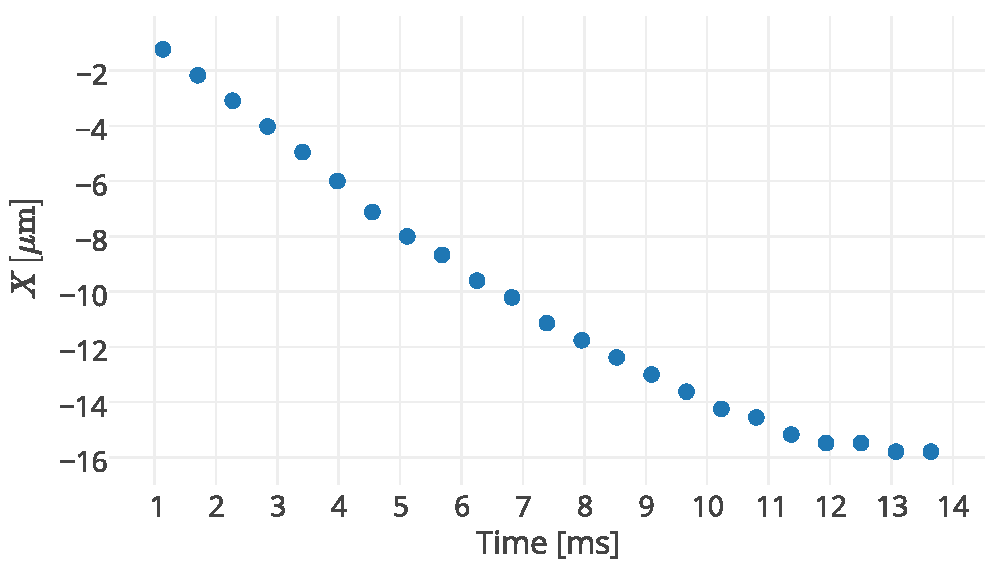
\includegraphics[width=8cm]{Plots/soliton_track.pdf}
	\caption{Calculated soliton position along the $x$ axis over the time.} \label{plot:soliton-xposition}
	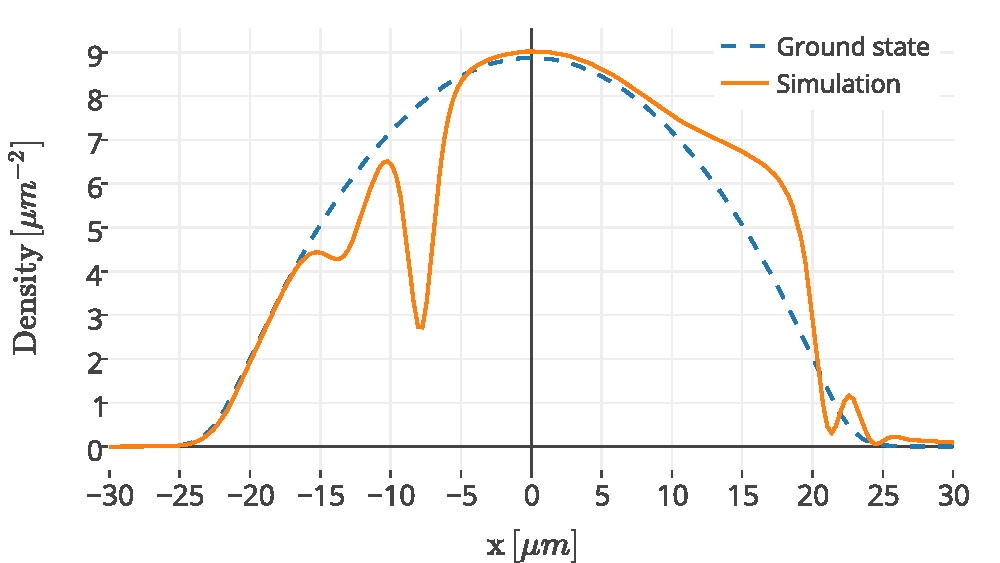
\includegraphics[width=8cm]{Plots/density_xprofile_5ms.pdf}
	\caption{Calculated ground state and particles density at $t = 5$~ms along the $x$ axis. The deep soliton is located at $x = -8 $~$ \mathrm{\mu m}$, in agreement with the experimental value~\citep{DSF00}. Other structures are visible from this figure: a shallow  dark soliton at $x = -14 $~$ \mathrm{\mu m}$ moving to the left; other excitations near $x = 20 $~$ \mathrm{\mu m}$ moving fast to the right.} \label{plot:density_5ms}
\end{figure}

The soliton speed is not the same throughout the BEC, as it depends on the particles density (Eq.~\eqref{eq:soliton-speed-density}). It is zero at the edge of the BEC, while it reaches its maximum at the center of the BEC. Indeed, rewriting Eq.~\eqref{eq:soliton-speed-density} as follows
\begin{equation}
\nu_s = \nu_0 \sqrt{1 - \frac{n - n_{min}}{n}},
\end{equation}
we see that $\nu_s$ goes to zero at the edge where both $n$ and $n - n_{min}$ go to zero, whereas the fraction $(n - n_{min}) / n$ reaches its lowest value at the center and $\nu_s$ is maximum. This implies that the soliton assumes a curved shape, whose
% clarify what I mean with curved shape
 curvature increases as the soliton travels far from the center. This feature of the soliton is observed both in the experiment and in our simulation (Fig.~\ref{plot:density-exp-sim}). 

In Fig.~\ref{plot:density_5ms}, the particles density profile along the $x$ axis is shown after $5$~ms from the phase imprinting. The deep soliton is located at $x = -8 $~$ \mathrm{\mu m}$, in agreement with the experimental value~\citep{DSF00}. Other structures are visible from this figure: a shallow  dark soliton at $x = -14 $~$ \mathrm{\mu m}$ moving to the left; other excitations near $x = 20 $~$ \mathrm{\mu m}$ moving fast to the right. These features are not well resolved in the experimental images, but they are in agreement with the simulations in~\citep{DSF00}.
\begin{figure}
\centering
\begin{tabular}{ccccc}
\subfloat[$1$ ms]{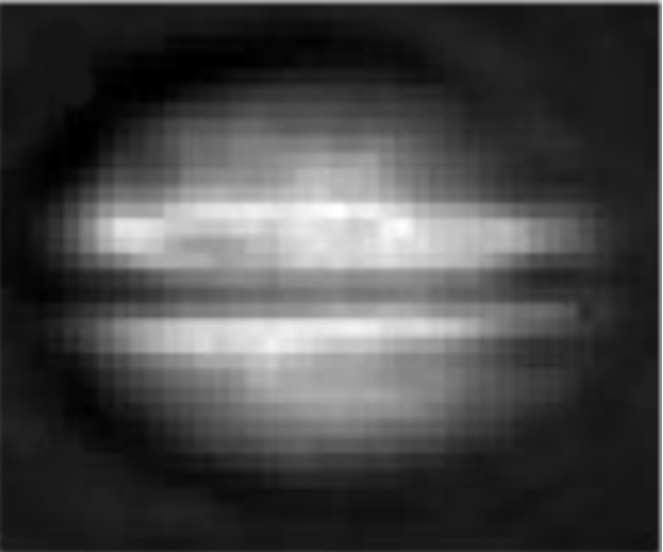
\includegraphics[width=1.9cm]{Plots/density_exp_1ms.pdf} \label{plot:density_exp_1ms}} & 
\subfloat[$2$ ms]{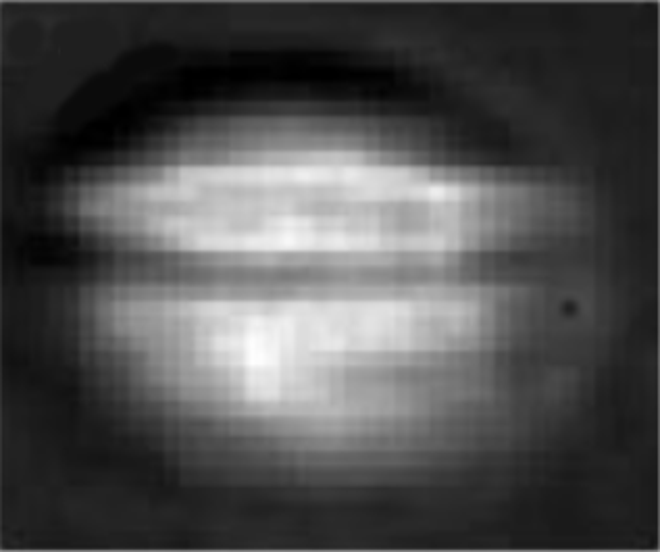
\includegraphics[width=1.9cm]{Plots/density_exp_2ms.pdf} \label{plot:density_exp_2ms}} & 
\subfloat[$5$ ms]{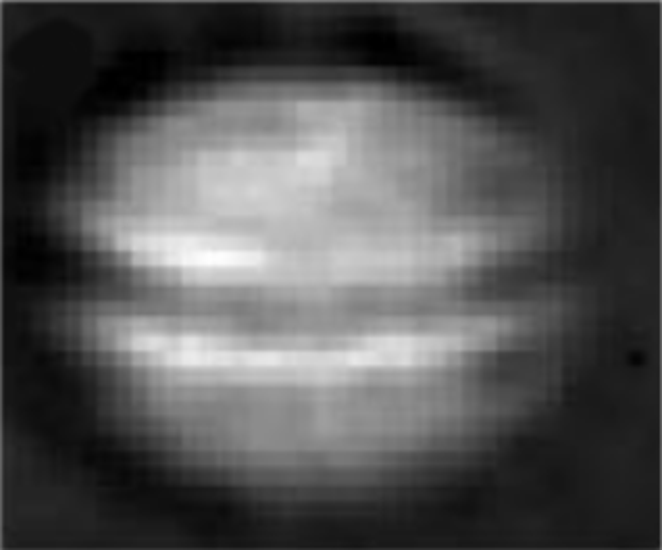
\includegraphics[width=1.9cm]{Plots/density_exp_5ms.pdf} \label{plot:density_exp_5ms}} & 
\subfloat[$7$ ms]{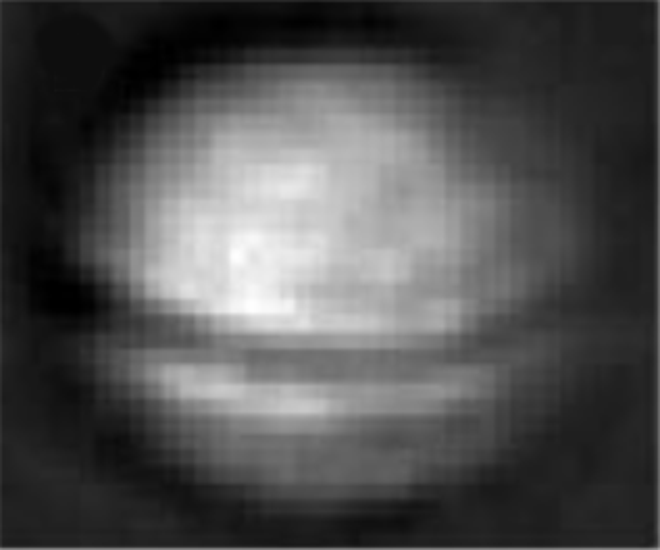
\includegraphics[width=1.9cm]{Plots/density_exp_7ms.pdf} \label{plot:density_exp_7ms}} &
\subfloat[$10$ ms]{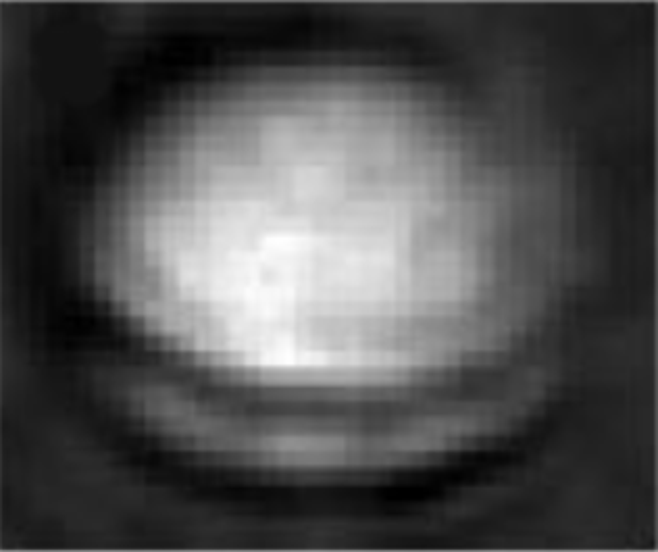
\includegraphics[width=1.9cm]{Plots/density_exp_10ms.pdf} \label{plot:density_exp_10ms}} \\
\subfloat[$1$ ms]{
\includegraphics[width=1.9cm]{Plots/density_hmap_1ms.pdf} \label{plot:density_sim_1ms}} & 
\subfloat[$2$ ms]{
\includegraphics[width=1.9cm]{Plots/density_hmap_2ms.pdf} \label{plot:density_sim_2ms}} & 
\subfloat[$5$ ms]{
\includegraphics[width=1.9cm]{Plots/density_hmap_5ms.pdf} \label{plot:density_sim_5ms}} & 
\subfloat[$7$ ms]{
\includegraphics[width=1.9cm]{Plots/density_hmap_7ms.pdf} \label{plot:density_sim_7ms}} &
\subfloat[$10$ ms]{
\includegraphics[width=1.9cm]{Plots/density_hmap_10ms.pdf} \label{plot:density_sim_10ms}} \\
\end{tabular}
\caption{Experimental images of the integrated BEC density ((a) to (e))~\citep{DSF00} and calculated density, from our simulation, ((f) to (j)) for various times after the phase imprinting. A positive density disturbance is created and moves rapidly in the $+x$ direction. A dark soliton is left behind moving in the opposite direction at significantly less than the speed of sound.} \label{plot:density-exp-sim}
\end{figure}


\begin{figure}[t]
\centering
\begin{tabular}{ccccc}
\subfloat[$14$ ms]{
\includegraphics[width=2cm]{Plots/density_hmap_14ms.pdf} \label{plot:density_sim_14ms}} & 
\subfloat[$17$ ms]{
\includegraphics[width=2cm]{Plots/density_hmap_17ms.pdf} \label{plot:density_sim_17ms}} & 
\subfloat[$18$ ms]{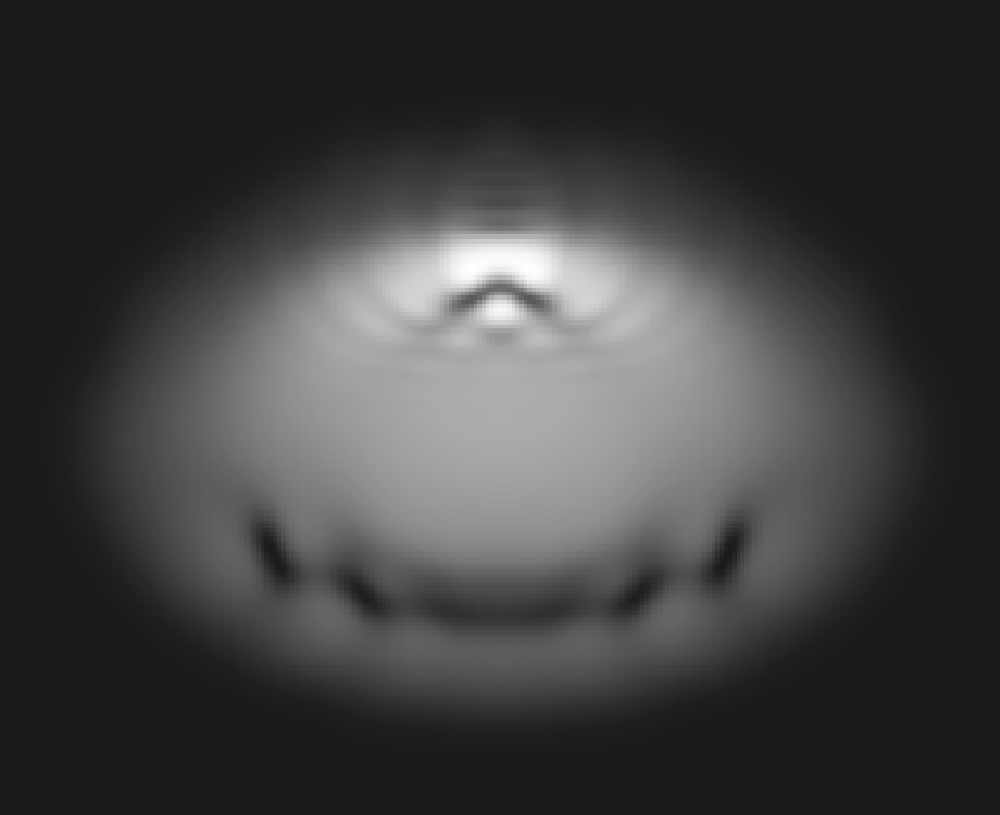
\includegraphics[width=2cm]{Plots/density_hmap_18ms.pdf} \label{plot:density_sim_18ms}} & 
\subfloat[$20$ ms]{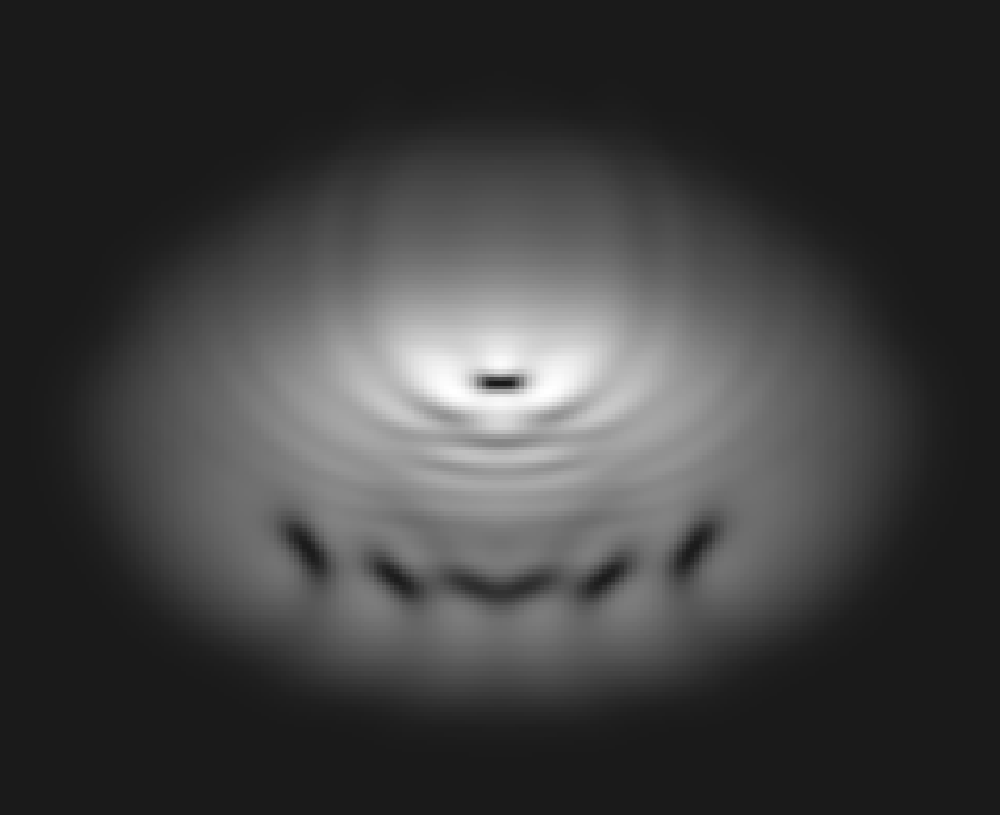
\includegraphics[width=2cm]{Plots/density_hmap_20ms.pdf} \label{plot:density_sim_20ms}} \\
\end{tabular}
\caption{Calculated particles density for various times after the soliton stops. These images show how the soliton breaks up.} \label{plot:density-breaksup}
\end{figure}

Since the external potential has a minimum, the soliton is expected to oscillate with a frequency of $\omega_s = \omega_x / \sqrt{2}$. This behaviour was also found by previous simulations~\citep{MLS99,BA98}. In our case, the soliton should stop after one--quarter of the oscillation time: $T_s/4 = \frac{\pi}{\sqrt{2} \omega_x} = 12.6 $~$ \mathrm{ms}$, which is in good agreement with our simulation (Fig.~\ref{plot:soliton-xposition}).

We were able to evaluate a quarter of period of the soliton and not the whole period because after the notch stops it breaks up, becoming rather perturbed (Fig.~\ref{plot:density-breaksup}). This behaviour is found also in the simulations carried out in~\citep{DSF00}. 
%%%%%%%%%%%%%%%%%%%%%% EXPLAIN WHY THE SOLITON DISAPPEAR %%%%%%%%%%%%%%%
%I guess this is because a soliton is well defined only on top of a "fat" and rather uniform BEC, while of course at the edges of the cloud the density goes to zero (so the interaction play a vanishing role there), and the density profile also changes very rapidly

In conclusion, though our simulation is based on the solution of the two--dimensional Gross--Pitaevskii equation, we were able to reproduce the results of both their experiment and simulation, which was based on the solution of the 3D Gross--Pitaevskii equation~\citep{DSF00}.

\chapter{Conclusion}
In this Thesis we developed a code for solving the time--dependent Schr\"odinger equation of a wave function in a two--dimensional space. The code implements a solver for quantum systems described by Hamiltonians with a static external potential and a self--interacting term. Furthermore, the code includes a solver for the imaginary time evolution, to approximate the ground state of the system.

This result has been obtained by extending  a recent work of Wittek and Cucchietti~\citep{Wittek20131165}, in which they developed a solver for a free quantum particle that scales to massively parallel computing clusters. The code implements the algorithm on four different kernels: two cache optimized kernels for central processing unit (CPU) -- one is further optimized to use the SSE instructions --, a kernel for general--purpose graphics processing unit (GPU) and a hybrid kernel that use both CPUs and GPUs. The algorithm is based on the second order of the Trotter--Suzuki approximation, which provides an accurate approximation of the evolution operator. Moreover, the approximation leads to an algorithm easy to parallelise that results in an efficient distribution of the workload across the nodes of a cluster. Indeed, the CPU kernels show a linear scaling of the throughput, so that doubling the number of cores, involved in the calculation, results in a halved time of execution. This can lead to very fast simulations on big clusters. On the other hand, GPU and hybrid kernels obtain better performances on a smaller scaled system, which makes them preferable on a single workstations.

We proved the accuracy of our code reproducing the results obtained by an experiment carried out at the National Institute of Standard and Technology (NIST)~\citep{DSF00}. We approximated the ground state of a Bose--Einstein condensate (BEC) of sodium atoms, confined in a magnetic trap, and simulated the evolution of the state that underwent on a phase imprinting. We were able to see the generation of a soliton and other excitations in agreement with the experimental observations.

We achieved this by mean of the approximation described in Ref.~\citep{PietroMassignan}. This approximation let us reduce the three dimensional Gross--Pitaevskii equation, which provides a model of the BEC, to a two dimensional model solvable by our code.

The software comes with the General Public License and it can be redistributed under the terms of this license. We developed an application programming interface (API) that exposes the function that performs the evolution. Furthermore, the CPU and SSE kernels are accessible from Python and MATLAB\footnote{For more information about how to get the code visit the web site https://github.com/peterwittek/trotter-suzuki-mpi.}.

A clear direction for future extensions of the code is the implementation of the nonlinear Schr\"odinger equation to all the kernels -- at the moment it is only supported on the CPU kernel. These would be useful in many fields of physics, for instance in ultracold atom physics, in which the Gross--Pitaevskii equation plays a major role in describing the systems. In this case, the phenomenology to be studied include vortexes, spin--orbit coupling~\citep{GS13} and quantum thermalization. Other applications may regards the simulations of cloak system and quantum holography.

The method used to rescale a three dimensional problem to  a two dimensional one may not be always applicable. This motivates the extension to three dimensions. The variety of possible decomposition strategies in this case is large, and a flexible implementation would be very useful to test out the performance of the different choices.

\appendix
\chapter{Reduction of dimension: constant spatial extent of the solution} \label{App:A}
The understanding of a phenomenon, in science, goes through the solution of a model. Very often this task is difficult or even impossible to accomplish without making some hypothesis that simplify the problem. The approach is to reduce the problem to solve simpler equations with fewer degrees of freedom. A good method is to identify the symmetries of the problem, and rewrite the equations in a new set of variables which make them decoupled. So that the dynamic can be solved for independent groups of variables or even be ignored for some of them, reducing the problem to a lower number of variables. For instance, the equations for the tri-dimensional dynamic of the two bodies problem can be written as a system of three independent equations, using the appropriate variables.

For many models this approach is not suitable, as the case of the Gross-Pitaevskii equation for a self-interacting BEC. Another procedure consist of making a posteriori (phenomenological) hypotheses, that let us to deal with a simpler problem with fewer variables. In this work we reduce a 3D Gross-Pitaevskii equation to a 2D equation, requiring that the solution of the 2D equation has the same spatial extent~\citep{PietroMassignan}.

The general $d$-dimensional Gross-Pitaevskii equation, with an anisotropic harmonic potential, is written as:
\begin{equation}
\imath \hbar \frac{\partial \psi(\textbf{r}, t)}{\partial t} = \left[ - \frac{\hbar^2}{2m} \sum_{i=1}^d \frac{\partial^2}{\partial x_i^2} + \frac{m}{2} \sum_{i=1}^d \omega_i^2 x_i^2 + U_0^{(d)} |\psi(\textbf{r}, t)|^2 \right] \psi(\textbf{r}, t),
\end{equation}
where the form of $U_0^{(d)}$ depends on the dimension of the problem; for $d=3$ we have:
\begin{equation}
U_0^{(3)} = \frac{4\pi \hbar^2 a_s}{m}.
\end{equation}

In the Thomas-Fermi approximation, the wave function of a stationary state satisfy the condition
\begin{equation}
|\psi_{TF}(\textbf{r})|^2 = \frac{\mu_{TF} - V(\textbf{r})}{U_0^{(d)}} \,\, \mathrm{if} \, \mu_{TF}  > V(\textbf{r})
\end{equation}
so, given the external potential, the spatial extent of the system is determined by the chemical potential $\mu_{TF}$. For an anisotropic harmonic potential, the spatial extent of a reduced system will be the same as the complete one if the chemical potential is the same.

Furthermore, in the Thomas-Fermi approximation it is possible to express the coefficient of the self-interaction as a function of the chemical potential, due to the normalization condition of the wave function, namely:
\begin{equation}
\begin{split}
N & = \int_V \mathrm{d}^d \textbf{r} \, |\psi_{TF}(\textbf{r})|^2 \\
& = \int_V \mathrm{d}^d \textbf{r} \, \frac{1}{U_0^{(d)}} \left[ \mu_{TF} - \frac{m}{2} \sum_{i=1}^d \omega_i^2 x_i^2 \right] \\
& = \frac{\mu_{TF}}{U_0^{(d)}} \left( \bar{R}_{TF} \right)^d \int_{S_1^{(d)}} \mathrm{d}^d \textbf{r} (1 - \textbf{r}^2) \\ 
& = \frac{\mu_{TF}}{U_0^{(d)}} \left( \bar{R}_{TF} \right)^d \frac{2\pi^{d/2}}{\Gamma(d/2)} \int_0^1 \mathrm{d}r \, r^{d-1} [1 - r^2] \\
& = \frac{\mu_{TF}}{U_0^{(d)}} \left( \bar{R}_{TF} \right)^d \frac{2\pi^{d/2}}{\Gamma(d/2)} \left( \frac{1}{d} - \frac{1}{d+2} \right) \\
& = \frac{\mu_{TF}}{U_0^{(d)}} \left( \bar{R}_{TF} \right)^d \frac{\pi^{d/2}}{\Gamma(d/2 + 2)}
\end{split}
\end{equation}
where $\bar{R}_{TF} = \sqrt{2\mu_{TF} / m \bar{\omega}^2}$ is the mean Thomas-Fermi radius, $\bar{\omega} = \sqrt[d]{\prod_{i=1}^d \omega_i}$ is the geometric mean of the frequencies and $S_1^{(d)}$ is the $d$-dimensional sphere.
This give us the formula
\begin{equation}
U_0^{(d)} = \frac{\mu_{TF}}{N} \left( \bar{R}_{TF} \right)^d \frac{\pi^{d/2}}{\Gamma(d/2 + 2)},
\end{equation}
that for $d=2$ gives
\begin{equation} \label{eq:self-interaction-2d}
U_0^{(2)} = \frac{\pi}{2} \frac{\mu_{TF}}{N} \left( \bar{R}_{TF} \right)^2.
\end{equation}

Combining Eq.~\eqref{eq:self-interaction-2d} and the constant of the chemical potential we can reduce the problem from three to two dimension. The resulting equation for the reduced system will be
\begin{equation}
\imath \hbar \frac{\partial \psi(\textbf{r}, t)}{\partial t} = \left[ - \frac{\hbar^2}{2m} \sum_{i=1}^2 \frac{\partial^2}{\partial x_i^2} + \frac{m}{2} \sum_{i=1}^2 \omega_i^2 x_i^2 + \frac{\pi}{2} \frac{\mu_{TF}}{N} \left( \bar{R}_{TF} \right)^2 |\psi(\textbf{r}, t)|^2 \right] \psi(\textbf{r}, t)
\end{equation}

\bibliographystyle{plain}
\bibliography{references}

%
\includepdf[pages={2-5}]{trotter-suzuki_nva.pdf}

\end{document}
